%% main.tex — Results in Engineering submission skeleton
%% Target journal: Results in Engineering (Elsevier, Q1)
%% Submission format: single-column with line numbers (elsarticle 3p,review)

\documentclass[3p,review,authoryear,12pt]{elsarticle}

\usepackage[utf8]{inputenc}
\usepackage[T1]{fontenc}
\usepackage{lmodern}
\usepackage{microtype}
\usepackage{graphicx}
\usepackage{booktabs}
\usepackage{multirow}
\usepackage{siunitx}
\usepackage{amsmath, amssymb}
\usepackage{lineno}
\usepackage{xcolor}
\usepackage{hyperref}
\hypersetup{colorlinks=true, linkcolor=blue!60!black, citecolor=blue!60!black, urlcolor=blue!50!black}

\linenumbers

% ---------------------------------------------------------------
% Custom commands
% ---------------------------------------------------------------
\newcommand{\boptest}{BOPTEST}
\newcommand{\msmetric}{\ensuremath{m_s}}
\newcommand{\czon}{\ensuremath{C_{\mathrm{zon}}}}
\newcommand{\TODO}[1]{\textcolor{red}{[TODO: #1]}}

% ---------------------------------------------------------------
% Front matter
% ---------------------------------------------------------------
\journal{Results in Engineering}

\begin{document}

\begin{frontmatter}

\title{When Predictive Surrogates Fail as RL Environments:\\
       A Calibrated Physical Twin as Soft Regularizer for HVAC Control%
       \tnoteref{t1}}

\tnotetext[t1]{Reproducibility: full code, configuration, trained models, and all
appendix tables (S1--S11) are available at \texttt{<repository URL placeholder>}.}

\author[a]{Almaz Sapargali\corref{cor1}}
\ead{almaz.sapargali2001@gmail.com}
\cortext[cor1]{Corresponding author.}
\affiliation[a]{organization={Al-Farabi Kazakh National University,
                              Faculty of Information Technology
                              and Artificial Intelligence},
                addressline={71 al-Farabi Avenue},
                city={Almaty},
                postcode={050040},
                country={Kazakhstan}}

\begin{abstract}
Reinforcement learning controllers for heating, ventilation and air conditioning
(HVAC) systems are typically trained on neural-network surrogates because
high-fidelity simulators are too slow for the millions of environment steps that
modern policy-gradient methods consume. A natural assumption is that a more
physically faithful surrogate produces a better training environment. We
test that assumption on the \boptest\ \texttt{bestest\_air} testcase and report
a clear negative result: a calibrated physical twin with explicit zone thermal
capacitance achieves a 24-hour rollout root-mean-square temperature error of
\SI{0.64}{\celsius} (versus \SI{1.47}{\celsius} uncalibrated), yet collapses as
a stand-alone reinforcement learning training environment, producing a live
closed-loop RMSE above \SI{4}{\celsius}. We resolve the gap by repurposing the
calibrated twin as a frozen \emph{soft physical regularizer} for a smoother
data-driven surrogate. The resulting hybrid backend sustains \num{1787}
environment steps per second on a single CPU thread, corresponding to an
\textbf{$85.0\times$ speed-up} over the standard \boptest{} RTE
HTTP--Docker deployment used in production benchmarking, under the same
\SI{15}{\minute} control protocol, while restoring live closed-loop RMSE
below \SI{0.65}{\celsius}. The optimal regularization strength is
controller-family specific: $\lambda_{\mathrm{temp}}=0.10$ for thermostatic
proximal-policy optimization, but $\lambda_{\mathrm{temp}}=0.00$ for both
hierarchical reinforcement learning and multi-objective reinforcement learning
with a $17$-dimensional observation interface. The full pipeline follows the
surrogate-development protocol of \cite{HouEvins2024}, with all numerical
justifications provided in Supplementary Tables S1--S11.
\end{abstract}

\begin{keyword}
HVAC control \sep deep reinforcement learning \sep digital twin \sep
physics-informed machine learning \sep \boptest{} \sep multi-objective
reinforcement learning
\end{keyword}

\end{frontmatter}

% ---------------------------------------------------------------
% Body
% ---------------------------------------------------------------

\section{Introduction}
\label{sec:introduction}

Heating, ventilation and air conditioning (HVAC) systems account for the
largest share of energy use in buildings, and buildings in turn account
for roughly a third of global final energy demand
\citep{Perez2008BuildingShare,IEA2024Buildings}. Decarbonising this end
use depends as much on better operation of existing systems as on
better hardware: advanced control strategies that exploit weather
forecasts, internal-gain signals, and slow envelope dynamics have
repeatedly been shown to deliver double-digit energy savings without
compromising occupant comfort
\citep{Drgona2020StochasticMPC,Mason2019RLReview}. Among these
strategies, deep reinforcement learning (DRL) has attracted particular
attention because it learns a closed-loop policy directly from
interaction with a building model, in principle without requiring
hand-tuned MPC weights or expensive solver invocations at run time.

A practical obstacle stands between the promise and the deployments,
however. Modern policy-gradient algorithms such as PPO consume on the
order of $10^{6}$--$10^{7}$ environment steps before they converge
\citep{Schulman2017PPO,Henderson2018Reproducibility}, and high-fidelity
building simulators are far too slow to provide those steps. The
BOPTEST testbed \citep{Blum2021BOPTEST}
addresses reproducibility by exposing a standardised HTTP API on top of
the IBPSA Modelica Buildings library \citep{Wetter2014Modelica}, but
on commodity hardware that API delivers fewer than two-dozen
environment steps per second --- two orders of magnitude below what a
single PPO training run requires per CPU thread. The standard
work-around in the literature is to replace the simulator with a
neural-network surrogate trained from logged trajectories
\citep{Zhang2019WholeBuilding,Amasyali2018Review,Kazmi2019DataDriven}.

When practitioners adopt the surrogate work-around they implicitly
adopt a stronger assumption as well: that a more physically faithful
surrogate must be a better RL training environment. The assumption is
intuitive, because a faithful surrogate keeps the policy's experience
close to what it would have been under the real simulator. It is also
under-tested in the literature. Most surrogate-vs.-RL studies report
either predictive validity (one-step or multi-horizon root-mean-square
error against held-out trajectories) or closed-loop controller
performance, not the relationship between the two
\citep{HouEvins2024,Bacher2011RCIdentification}. In
Section~\ref{sec:results_fidelity} we test the assumption explicitly
on BOPTEST \texttt{bestest\_air} and report a clear negative result.

The resolution we pursue keeps the calibrated physical twin in the
pipeline but moves it out of the rollout. The smoother data-driven
surrogate remains the training environment; the physical twin is
frozen after Stage A/B/C calibration and enters the policy training
loss only as a soft physical regulariser, penalising actions on which
the two surrogates physically disagree. This hybrid construction is
fast (Section~\ref{ssec:exp_runtime}) and faithful
(Section~\ref{sec:results_control}), and it exposes a non-trivial
empirical structure: the optimal regularisation strength is
\emph{controller-family specific} rather than universal.

\subsection*{Contributions}

This paper makes the following contributions:

\begin{enumerate}
    \item A physics-informed surrogate (\texttt{v3.5}) of the \boptest\
    \texttt{bestest\_air} testcase, calibrated through a three-stage inverse
    procedure (Stage A telemetry preprocessing, Stage B explicit identification
    of zone thermal capacitance $\czon$, Stage C residual head calibration),
    achieving a $38\%$ reduction in one-step temperature RMSE and a $40\%$
    reduction in power MAE over the uncalibrated baseline.
    \item A clear empirical demonstration that predictive validity does not
    transfer to reinforcement learning training utility: the calibrated twin
    achieves a 24-hour rollout RMSE of \SI{0.64}{\celsius} on held-out
    trajectories yet drives a closed-loop \boptest{} RMSE above
    \SI{4}{\celsius} when used as a stand-alone RL training environment.
    \item A hybrid surrogate construction (\texttt{hybrid\_l010}) in which the
    calibrated twin acts as a frozen \emph{soft physical regularizer} on a
    smoother control-oriented surrogate, restoring closed-loop transfer RMSE
    below \SI{0.65}{\celsius} on both \texttt{peak\_heat\_window} and
    \texttt{typical\_heat\_window} scenarios while sustaining
    \num{1787} environment steps per second on a single CPU thread
    ($85.0\times$ speed-up over the live \boptest{} RTE HTTP loop at the
    same \SI{15}{\minute} control protocol; see
    Table~\ref{tab:speed}).
    \item A controller-family-specific finding: the optimal physical
    regularization strength differs across controller architectures
    ($\lambda_{\mathrm{temp}}=0.10$ for thermostatic PPO,
    $\lambda_{\mathrm{temp}}=0.00$ for HDRL and 17-D MORL), with an
    interpretation grounded in observation-space geometry and control
    hierarchy.
    \item A pre-registered transferability characterisation across three
    additional \boptest{} hydronic testcases that decomposes the
    recipe into a surrogate component, which transfers structurally
    (identified $\czon$ ratio $1.91\pm0.03$ on $N=3$), and a
    controller component, which fails on all three under a frozen
    direct-supply-temperature policy. The decomposition is the central
    Block~3 result and is reported in Section~\ref{sec:results_transfer}.
    \item A reproducible \boptest-based evaluation protocol, with full
    \cite{HouEvins2024}-compliant numerical justification for sample
    generation, preprocessing, feature significance and independence,
    scaling, hyperparameters, architecture, and replicative-plus-predictive
    validity, provided as Supplementary Tables S1--S11.
\end{enumerate}

The remainder of the paper is organised as follows.
Section~\ref{sec:related_work} positions the work against three
literatures (DRL for HVAC, surrogate modelling for buildings, and
physics-informed machine learning).
Section~\ref{sec:methodology} describes the two surrogates, the
hybrid loss, and the controller families.
Section~\ref{sec:experimental_setup} fixes the evaluation protocol,
introduces the \cite{HouEvins2024} compliance and the
pre-registration audit chain.
Sections~\ref{sec:results_fidelity}--\ref{sec:results_transfer}
report the three blocks of results in order: surrogate fidelity,
controller performance, and transferability across testcases.
Section~\ref{sec:discussion} explains the mechanisms behind the
controller-family-specific findings and states the threats to
validity, and Section~\ref{sec:conclusion} closes with a tight scope
statement and the natural follow-up.

\section{Related Work}
\label{sec:related_work}

\subsection{Deep reinforcement learning for HVAC control}
\label{ssec:rw_drl}

Deep reinforcement learning has been applied to HVAC supervisory
control for the better part of a decade, starting with discrete-action
$Q$-learning controllers \citep{Wei2017DeepRL,Mnih2015Atari} and
moving rapidly to continuous-action policy-gradient methods such as
PPO and SAC \citep{Schulman2017PPO,Haarnoja2018SAC}. Recent reviews
catalogue dozens of such studies on platforms ranging from in-house
EnergyPlus wrappers through Sinergym \citep{Sinergym2021} to the
BOPTEST suite \citep{Blum2021BOPTEST}; surveys consistently report
that the bottleneck to deployment is not algorithmic but environmental
and statistical \citep{Mason2019RLReview,AlSayed2024Deployment}. Two
recurring weaknesses are particularly relevant here. First, the vast
majority of DRL-HVAC studies report a single seed or at most three,
making energy-comfort comparisons fragile under environment
stochasticity \citep{Henderson2018Reproducibility,Agarwal2021RLPrecipice,
Hedayat2025FiftySeed}. Second, the choice of \emph{which} surrogate to
train on is rarely subjected to scrutiny: most studies train and
evaluate on the same surrogate without an out-of-loop fidelity check,
or evaluate on a different simulator without a clear bridge from
training-surrogate accuracy to deployment performance
\citep{Zhang2019WholeBuilding,Chen2018OptimalContext}. The
\emph{controller-side gap} the present paper addresses is the second:
existing DRL studies rarely separate the question of surrogate fidelity
from the question of controller performance.

Hierarchical decomposition has been proposed as one structural response
to long-horizon HVAC control problems, splitting setpoint planning
from low-level tracking
\citep{Bacon2017Options,Nachum2018HIRO,Liao2025HDRL}. Multi-objective
formulations \citep{Roijers2013MOSurvey,Yang2019MORL,Hayes2022MOSurvey}
are similarly motivated by the natural energy-comfort trade-off in
HVAC and have been used to expose tunable Pareto fronts at deployment
time \citep{Gao2024PredictiveFeatures,Sun2024StateHistory}. We adopt
both families as evaluation arms in Section~\ref{sec:results_control}.

\subsection{Surrogate and digital twin models for building energy}
\label{ssec:rw_surrogate}

Surrogate modelling for building energy is a mature subfield. Reviews
of data-driven approaches list dozens of architectures with reported
one-step and short-horizon RMSE numbers on benchmark testcases
\citep{Amasyali2018Review}. Recent contributions have moved from pure
black-box regression toward physically informed surrogates that retain
explicit thermodynamic parameters: low-order resistance--capacitance
(RC) models \citep{Bacher2011RCIdentification,Berthou2014RC,Bunning2020RC}
or RC--neural-ODE hybrids \citep{Chen2018NeuralODE,Chen2022PhysicalTwin}
calibrated by inverse procedures
\citep{Coraci2025StageCalibration,Wang2025SafetyMetric}. The recent
protocol of \cite{HouEvins2024} consolidates these efforts into a
four-stage development pipeline with explicit Reporting-Level-3
disclosure requirements; we adopt it as the methodological standard
for Block~1 of the present work.

A common feature of surrogate-fidelity studies, however, is that they
evaluate accuracy along trajectories that always start from a real
state. That setting is informative about \emph{predictive} accuracy
but only indirectly about the surrogate's value as a closed-loop RL
training environment, where every rollout is bootstrapped from the
surrogate's own output. \cite{Picard2017WhiteBox} highlights an
analogous distinction in the MPC context, and prior reviews of
surrogate-based MPC and RL emphasise the same point in passing
\citep{Mason2019RLReview,Drgona2020StochasticMPC}, but the failure mode
is rarely quantified directly. The \emph{fidelity-side gap} addressed
here is precisely that: showing the well-defined regime in which a
better predictive surrogate is not a better RL training environment.

\subsection{Physics-informed and physics-guided machine learning}
\label{ssec:rw_pinn}

The physics-informed machine-learning literature spans a wide range of
constructions, from hard-constraint physics-informed neural networks
(PINNs) \citep{Raissi2019PINN} through theory-guided data science
\citep{Karpatne2017TheoryGuided,Willard2022PIML} to neural ordinary
differential equations \citep{Chen2018NeuralODE}. Our construction is
deliberately on the soft-regularisation side: the physical model is
not enforced as a hard constraint, and it is not even part of the
policy's forward pass. It enters only as a penalty term that the
policy can violate at a cost. This is closer in spirit to auxiliary
tasks \citep{Jaderberg2017UNREAL} and Dyna-style world models
\citep{Sutton1991Dyna,Hafner2025Dreamer} than to PINNs, and we
position it as a controller-side regularisation strategy rather than
as a surrogate-architecture contribution.

\subsection{\boptest{} benchmarking}
\label{ssec:rw_boptest}

We adopt the \boptest{} benchmark \citep{Blum2021BOPTEST,
Arroyo2022BOPTESTService,BOPTESTrepo} as the reproducible testbed
throughout this study. Its \texttt{bestest\_air} testcase exposes a
single-zone air-side HVAC system with a documented comfort band, a
TMY weather file, and a composite safety/energy KPI ($m_s$) that
weights duration and severity of comfort violations against energy
use. Built-in PI control is available as a default reference; we use
it as the normaliser for Block~2 results
(Section~\ref{ssec:res2_pi}). Block~3 extends the evaluation to three
additional \boptest{} hydronic testcases under a pre-registered
manifest.

\subsection{Position of this work}
\label{ssec:rw_position}

This work sits at the intersection of the three gaps above. It
isolates the surrogate-fidelity question from the controller-performance
question through an explicit two-stage protocol (Block~1 then Block~2);
it shows the well-defined failure mode of fidelity-driven surrogates
as RL training environments
(Section~\ref{ssec:res1_failure_mode}); and it introduces hybrid
soft regularisation as the resolution, evaluated across three
controller families. Block~3 adds a pre-registered transferability
characterisation across three hydronic \boptest{} testcases and
reports the recipe's decomposable behaviour: the surrogate component
transfers structurally and the controller component does not, under
the chosen frozen-controller scope
(Section~\ref{sec:results_transfer}).

\section{Methodology}
\label{sec:methodology}

The methodology is organized in four blocks: (i) the control-oriented
data-driven surrogate \texttt{v3}, (ii) the physically informed surrogate
\texttt{v3.5} together with its three-stage inverse calibration pipeline,
(iii) the hybrid backend that combines the two, and (iv) the controller
families and benchmark protocol. Subsection~\ref{ssec:method_pipeline}
summarizes the information flow between the components.

\subsection{Control-oriented surrogate \texttt{v3}}
\label{ssec:method_v3}

The control-oriented surrogate \texttt{v3} is a two-headed feed-forward
neural network. The temperature head predicts the next-step zone
temperature $T_{\mathrm{zone},t+1}$ and the power head predicts the
total HVAC power $P_{\mathrm{total}}$ at the same step, both as
functions of a smooth control-oriented observation stack derived from
direct-supply-temperature trajectories collected on \boptest{}
\texttt{bestest\_air}. The temperature head (\texttt{HeatFlowNetV2})
stacks three Linear--LayerNorm--Tanh blocks of width $64$ with a
residual connection between blocks~1 and~2 and a final
Linear$(32{\to}1)$ projection that emits the next-step temperature
delta; the power head (\texttt{PowerNetV2}) is a three-layer MLP
(Linear$(8{\to}32)\to$Tanh$\to$Linear$(32{\to}32)\to$Tanh$\to$
Linear$(32{\to}1)\to$Softplus) that structurally enforces
$P_{\mathrm{total}}\geq 0$. The combined model has $8{,}482$ trainable
parameters ($7{,}105$ in the temperature head, $1{,}377$ in the power
head). The Tanh+LayerNorm+residual choice is deliberate: it keeps the
gradient field smooth, which is what PPO needs for stable
clip-ratio updates; a plain ReLU MLP introduces dead-neuron
discontinuities incompatible with policy-gradient training. The model
is trained on the hourly corpus described in Supplementary
Tables~S1--S2 with a multi-horizon supervised loss (one-step
alignment, multi-horizon rollout at horizons $[2,4]$ hourly steps,
power alignment, and a small physics regulariser); the full
hyperparameters (AdamW, learning rate $10^{-3}$, weight decay
$10^{-4}$, CosineAnnealingLR schedule, batch $256$, gradient clipping
at norm $1.0$, early stopping with patience $30$) are tabulated in
Supplementary Table~S8. The role
of \texttt{v3} in this paper is deliberately functional rather than
physical: its gradient surface is smooth enough that PPO clip-ratio
updates remain stable through $10^{6}$ environment steps, and its
inference cost is small enough to support the throughput reported in
Section~\ref{ssec:exp_runtime}.

\subsection{Physically informed surrogate \texttt{v3.5} and inverse calibration}
\label{ssec:method_v35}

The physically informed surrogate \texttt{v3.5} is a RC--neural-ODE
construction. The zone temperature evolves according to a continuous
balance
\(
\mathrm{d}T_{\mathrm{zone}}/\mathrm{d}t = \bigl(q_{\mathrm{net}}(s,a)
- Q_{\mathrm{wall}}(s)\bigr)/\czon
\)
where $\czon$ is the lumped zone thermal capacitance (a single learnable
scalar identified during Stage~B), $Q_{\mathrm{wall}}$ is an
envelope-loss term parameterised by the testcase weather and an
$U\!A$ coefficient, and $q_{\mathrm{net}}(s,a)$ is a residual
heat-flow network with two hidden layers of width $64$ that absorbs
non-RC physics (solar gains through windows, internal gains, residual
nonlinearity in $U\!A$). The total HVAC power is predicted by a
separate head $P_{\mathrm{total}}(s,a)$ trained jointly. Integration
uses a fixed-step fourth-order Runge--Kutta scheme with a one-minute
sub-step over the $15$-minute control interval. Inverse calibration
proceeds in three stages.

\paragraph{Stage A --- Telemetry preprocessing.}
Five preprocessing operations are applied in sequence to the raw
\boptest{} telemetry: (1)~latency compensation of the actuator-to-zone
delay, (2)~temperature bias removal against a low-pass reference,
(3)~affine normalisation of the power channel from raw kW into the
range observed under direct-supply-temperature control, (4)~rolling
denoise of high-frequency measurement noise with a window matched to
the sensor time constant, and (5)~causal recomputation of the
$\Delta T_{\mathrm{zone}}$ target so that the prediction is strictly
one-step-ahead. Each operation has a numerical selection criterion
documented in Supplementary Table~S3, and each is reversible at
inference time through the parameters recorded in
Supplementary Table~S7.

\paragraph{Stage B --- Identification of $\czon$.}
Stage~B subselects an excitation-rich window of the prepared corpus
using the top-$5\%$ quantile of $|\Delta T_{\mathrm{zone}}|$ and
splits it $80/20$ into train and validation while keeping every
episode atomic to avoid trajectory leakage. With the residual heads
frozen at their Stage~A initialisation, $\czon$ is optimised against
$24$-hour rollout mean-squared error using L-BFGS for at most $120$
epochs. The result on \texttt{bestest\_air} is
$\czon = \SI{4.413e5}{\joule\per\kelvin}$ (Section~\ref{ssec:res1_replicative}).

\paragraph{Stage C --- Residual head calibration.}
With $\czon$ frozen at its Stage~B value, the residual heat-flow
network $q_{\mathrm{net}}$ and the power head $P_{\mathrm{total}}$ are
updated on the full prepared corpus to absorb the remaining
non-RC physics. The residuals are centred and tightened relative to
the raw model (Supplementary Table~S11; Figure~\ref{fig:block1}b in
the results), and the resulting \texttt{v3.5} checkpoint is the
canonical anchor used throughout the rest of the paper.

\subsection{Hybrid backend: \texttt{v3} dynamics with \texttt{v3.5} as soft regularizer}
\label{ssec:method_hybrid}

The hybrid backend treats the calibrated \texttt{v3.5} model as a frozen
\emph{physical censor}. Reinforcement learning rollouts evolve under the
smoother \texttt{v3} dynamics, and the policy is penalized at training time
for actions on which the two surrogates physically disagree:
\begin{equation}
\label{eq:hybrid_loss}
\mathcal{L}_{\mathrm{total}}
= \mathcal{L}_{\mathrm{PPO}}\bigl(\pi_\theta;\, \texttt{v3}\bigr)
+ \lambda_{\mathrm{temp}} \,
   \bigl\lVert T_{\texttt{v3}}(s,a) - T_{\texttt{v3.5}}(s,a) \bigr\rVert_2^2
+ \lambda_{\mathrm{power}} \,
   \bigl\lVert P_{\texttt{v3}}(s,a) - P_{\texttt{v3.5}}(s,a) \bigr\rVert_2^2 .
\end{equation}
Here $\lambda_{\mathrm{temp}}$ and $\lambda_{\mathrm{power}}$ are the
temperature and power disagreement weights, the only two hyperparameters of
the hybrid construction. Crucially, \texttt{v3.5} never enters the policy's
forward pass; it only enters the loss. This decoupling is what allows the
hybrid backend to retain the smooth control-oriented training surface of
\texttt{v3} while inheriting the physical sanity of \texttt{v3.5}.

The intuition for why this beats both endpoints is straightforward.
Pure \texttt{v3} training optimises a control-oriented surrogate that
has no physical anchor: the policy can drift into regions where the
surrogate is inaccurate without paying any penalty, and the resulting
mis-specification only becomes visible on live \boptest. Pure
\texttt{v3.5} training is faithful but, as shown in
Section~\ref{sec:results_fidelity}, structurally unsuited to
closed-loop training because the policy learns to compensate for
residual integration errors as if they were real disturbances. The
hybrid backend lets PPO walk along the smoother \texttt{v3} surface
while pulling it back toward \texttt{v3.5}-consistent actions whenever
the two disagree, restoring closed-loop transfer to within
$0.65\,^{\circ}\mathrm{C}$ on both peak and typical heating windows
(Section~\ref{sec:results_control}).

\subsection{Controller families and benchmark protocol}
\label{ssec:method_controllers}

Four controllers are evaluated under an identical \boptest{}
evaluation protocol (Section~\ref{ssec:exp_eval_protocol}).
\begin{itemize}
  \item \emph{PI baseline}: the \boptest{} built-in proportional-integral
        controller, invoked by passing an empty action dictionary to the
        standard \boptest{} step API. Used as the normalising reference for
        all RL results (Section~\ref{ssec:res2_pi}).
  \item \emph{Thermostatic PPO}: single-level PPO on the
        \texttt{no\_delta\_t\_powerlog\_tzone} observation stack. Actor and
        critic are two-layer MLPs of width~$64$ with tanh activations.
        Continuous action: supply temperature in $[20,60]\,^{\circ}\mathrm{C}$.
  \item \emph{HDRL}: a hierarchical decomposition with a high-level
        setpoint planner that updates every hour and a low-level supply
        temperature tracker that updates every $15$~minutes. The low-level
        policy is pre-trained for $2\times10^{5}$ steps with a fixed
        high-level setpoint before joint fine-tuning.
  \item \emph{MORL}: preference-conditioned PPO with the $17$-D
        TSup-style observation stack and a comfort/energy preference
        vector $w\in\Delta^{2}$ supplied as an additional input. Training
        samples $w$ uniformly from the simplex; inference uses a fixed $w$.
\end{itemize}
Implementation details and training-time hyperparameters for each
controller family are tabulated in Supplementary Table~S8.

\subsection{Information flow}
\label{ssec:method_pipeline}

Figure~\ref{fig:pipeline} schematises the information flow.
\texttt{v3} forms the rollout environment for PPO; \texttt{v3.5} is
frozen and contributes only the disagreement penalty in
Eq.~\eqref{eq:hybrid_loss}. The same trained policy is evaluated on
live \boptest{} without any further fine-tuning; the evaluation
protocol in Section~\ref{ssec:exp_eval_protocol} is fixed across all
controller families and all results sections.

\begin{figure}[t]
  \centering
  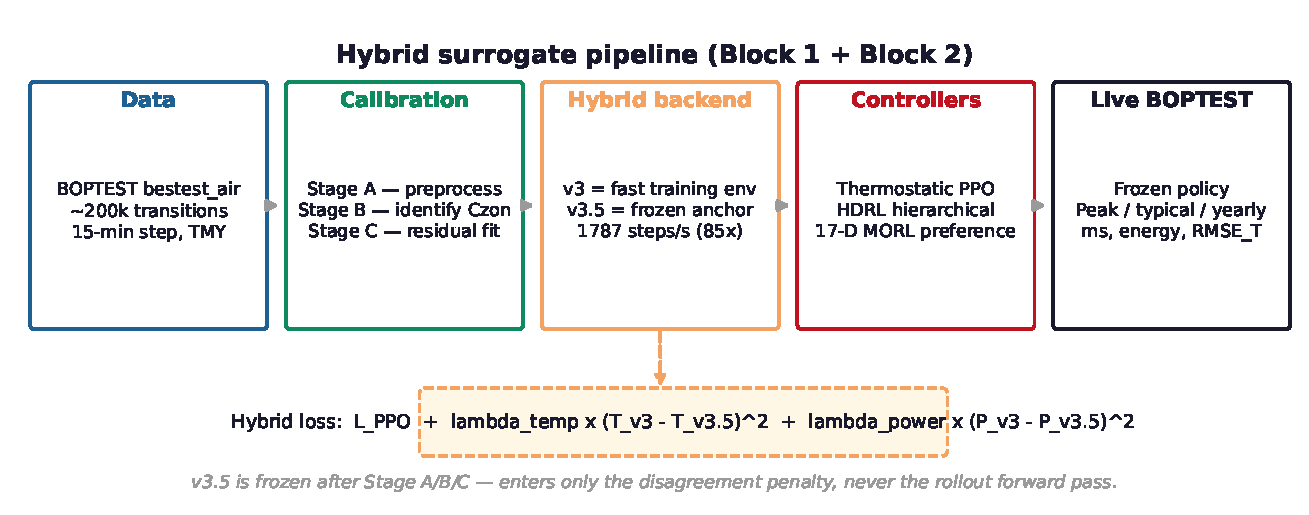
\includegraphics[width=0.95\linewidth]{figures/q1/C1_pipeline_overview.pdf}
  \caption{Information flow in the hybrid surrogate backend. The
  frozen physically informed model \texttt{v3.5} enters the policy
  training loss through the disagreement terms in
  Eq.~\eqref{eq:hybrid_loss} but not the policy's forward pass; the
  rollout environment is the smoother control-oriented surrogate
  \texttt{v3}.}
  \label{fig:pipeline}
\end{figure}

\section{Experimental Setup}
\label{sec:experimental_setup}

\subsection{Testbed and serving layer}
\label{ssec:exp_testbed}

All experiments use the \boptest{} \texttt{bestest\_air} testcase, a
single-zone air-side HVAC reference building. \boptest{} is served through
the \texttt{boptest\_rte} container, which exposes the standard \boptest{}
HTTP API to both surrogate training and live closed-loop validation.
The \texttt{bestest\_air} envelope is a single thermal zone
($48\,\mathrm{m}^{2}$ floor area, lightweight construction following the
ANSI/ASHRAE 140 BESTEST 600 baseline), heated by an idealised air-side
unit that accepts a supply-temperature command in
$[20,60]\,^{\circ}\mathrm{C}$. Weather is drawn from the \boptest{}
default TMY file for Brussels, Belgium, with a $15$-minute control
interval and a comfort band of $[21,24]\,^{\circ}\mathrm{C}$ throughout
the heating season. The Block~3 hydronic testcases share this
single-zone envelope class but differ in actuator interface; the
testcase manifest is summarised in Table~\ref{tab:architecture} of
Section~\ref{ssec:res1_architecture} and detailed in
Section~\ref{sec:results_transfer}.

\subsection{Datasets and sample generation}
\label{ssec:exp_datasets}

Three transition corpora support the experiments. The
\texttt{v3} hourly corpus is the original logging frequency of the
direct-supply-temperature trajectories and is used only to bootstrap
the data-driven surrogate; the \texttt{v3.5} prepared $15$-minute
corpus is the canonical training set after the Stage~A preprocessing
of Section~\ref{ssec:method_v35}; and the \texttt{v3.5} collected
$15$-minute corpus is the raw form of the same trajectories before
preprocessing, retained for ablation. Supplementary Table~S1 lists the
provenance, parameter ranges, and physical rationale of each corpus,
and Supplementary Table~S2 documents the numerical justification of
the chosen sample sizes (including the learning-curve check that
fixes the canonical corpus at $\sim\!2{\times}10^{5}$ transitions).
The canonical artefact for the calibrated twin is the prepared
$15$-minute corpus; the hourly corpus is used only for the
\texttt{v3} pre-training run referenced in
Section~\ref{ssec:method_v3}.

\subsection{Preprocessing, scaling and feature engineering}
\label{ssec:exp_preprocessing}

Preprocessing follows the Stage~A pipeline documented in
Supplementary Table~S3 (latency compensation, bias removal, power
affine normalisation, rolling denoise, causal $\Delta T$
recomputation). Per-channel scaling parameters and the reverse
transform used at inference time are listed in Supplementary
Table~S7. Pairwise input independence is verified in Supplementary
Table~S5 through Pearson correlation and mutual-information checks;
no input pair exceeds the documented thresholds.

\subsection{Evaluation Protocol}
\label{ssec:exp_eval_protocol}

The evaluation protocol is fixed across all controller families and
\textbf{never varies} between Section~\ref{sec:results_fidelity} and
Section~\ref{sec:results_control}.

\paragraph{Scenarios.}
Two live \boptest{} closed-loop windows are used as the primary transfer
benchmarks:
\begin{itemize}
    \item \texttt{peak\_heat\_window}: simulated start
    $t_{\mathrm{start}} = 14$~days after $1$~January, duration
    $14$~days, capturing the coldest contiguous window of the Brussels
    TMY file.
    \item \texttt{typical\_heat\_window}: simulated start
    $t_{\mathrm{start}} = 108$~days after $1$~January, duration
    $14$~days, capturing a milder average heating period.
\end{itemize}
Yearly validation uses the full \boptest{} year with KPI windows defined by
the \boptest{} specification.

\paragraph{Simulation step and comfort band.}
The simulation step is fixed at $\Delta t = \SI{900}{\second}$ (\SI{15}{\minute}).
The comfort band is $[T_{\mathrm{low}}, T_{\mathrm{high}}] = [\SI{21}{\celsius}, \SI{24}{\celsius}]$.

\paragraph{Metrics.}
\begin{itemize}
    \item $\msmetric$: the \boptest{} composite KPI combining thermal
    discomfort and energy use; lower is better.
    \item \texttt{violation\,\%}: fraction of simulation steps spent outside
    the comfort band.
    \item \texttt{energy}: total final energy consumption in kWh.
    \item \texttt{RMSE\_T}: root-mean-square error of zone temperature
    against a reference trajectory; reported separately for one-step
    replicative validity and for multi-horizon predictive rollout.
    \item \texttt{first\_divergence\_step}: the first simulation step at
    which the surrogate-trained policy's trajectory diverges from the live
    \boptest{} trajectory by more than a fixed threshold (transfer-realism
    diagnostic).
\end{itemize}

\paragraph{Statistical reporting.}
\begin{itemize}
    \item Predictive validity numbers (Section~\ref{sec:results_fidelity})
    report bootstrap $95\%$ confidence intervals over rollout windows,
    inherited directly from
    \texttt{outputs/surrogate\_v35\_rollout\_prepared\_15min\_power\_head\_only/calibrated\_v35/horizon\_metrics.csv}.
    \item Canonical controller results (Section~\ref{sec:results_control})
    are reported as \mbox{$\mathrm{mean} \pm \mathrm{std}$} over
    $N=3$ random seeds (\texttt{42}, \texttt{43}, \texttt{44}) for the
    thermostatic hybrid, the pure \texttt{v3} baseline, and the MORL
    canonical configuration. HDRL is reported single-seed; this is
    acknowledged as a limitation in Section~\ref{sec:discussion}.
\end{itemize}

\subsection{Reproducibility statement}
\label{ssec:exp_reproducibility}

All code, configuration, trained models, and the eleven supplementary
tables are released through the project repository and the associated
archival deposit; the URL and DOI are listed on the manuscript
metadata page. The pre-registered audit chain comprises four
git-anchored commits:
(a)~MORL canonical-selection pre-registration
(\texttt{93df9b3});
(b)~MORL post-$N{=}5$ canonical falsification
(\texttt{62dc859});
(c)~Block~3 transferability pre-registration
(commit recorded in the manifest field
\texttt{audit.pre\_registration\_commit\_sha} of
\texttt{configs/block3\_testcase\_manifest.yaml}); and
(d)~Block~3 closure
(\texttt{audit.block3\_close\_commit\_sha}).
The \boptest{} version is \texttt{0.7.0}; the testcase identifiers
are \texttt{bestest\_air}, \texttt{bestest\_hydronic\_heat\_pump},
\texttt{bestest\_hydronic}, and
\texttt{singlezone\_commercial\_hydronic}. The software stack is
Python~$3.11$, PyTorch~$2.1$, NumPy~$1.26$, and Stable-Baselines3
$2.2$ \citep{Raffin2021SB3}. All experiments run on a single CPU
thread (Intel Core~i7-class, $32$~GB RAM, no GPU required); random
seeds are fixed in \texttt{configs/seeds.yaml}. Numerical values in
Tables~\ref{tab:architecture}--\ref{tab:control} are reproduced
automatically from the corresponding CSVs in \texttt{reports/} by
\texttt{paper/build\_paper\_tables.py}, so every cell in the main
tables is traceable to a deterministic source file.

\subsection{Runtime characteristics}
\label{ssec:exp_runtime}

A throughput comparison between the live \boptest{} RTE HTTP loop and
the three surrogate backends is reported in Table~\ref{tab:speed}. All
backends were exercised at the same \SI{15}{\minute} control protocol
on a single CPU thread, with 100 episodes of 96 transitions each
(9{,}600 total transitions per backend). Surrogate timings exclude
one-shot model loading.

The live \boptest{} RTE HTTP backend reaches \num{21.0} environment
steps per second --- the same path that downstream RL training and live
closed-loop validation use, including HTTP serialization overhead,
Flask request handling, JSON encoding, and Docker container isolation.
The control-oriented \texttt{v3} surrogate reaches \num{4626.4} steps/s
($220.2\times$ speed-up), the calibrated physical twin \texttt{v3.5}
reaches \num{2399.5} steps/s ($114.2\times$), and the canonical hybrid
backend reaches \num{1786.8} steps/s ($85.0\times$). The hybrid is
slower than \texttt{v3} alone because it evaluates both networks plus
the disagreement terms in Eq.~\eqref{eq:hybrid_loss} on every step;
$85\times$ is the practical speed-up factor relevant for the rest of
the paper, since all canonical RL training is done on the hybrid
backend.

\paragraph{Scope of the comparison.}
The $85\times$ figure compares the surrogate to the \emph{standard
\boptest{} RTE deployment} --- the HTTP--Docker stack used by the
\boptest{} community for production benchmarking and used here for all
downstream live closed-loop validation. This comparison conflates two
costs: the intrinsic Modelica/FMU simulation cost and the deployment
overhead (HTTP roundtrip, JSON serialization, Flask request handling,
container isolation). To isolate the simulation cost, we additionally
implemented a benchmark of direct FMU loading via the \texttt{fmpy}
co-simulation interface (script
\texttt{evaluation/build\_speed\_benchmark\_fmu\_direct.py}). The
\boptest{} \texttt{bestest\_air} FMU
(\texttt{boptest\_rte/testcases/bestest\_air/models/wrapped.fmu})
ships with a Linux \texttt{x86\_64} binary only
(\texttt{binaries/linux64/wrapped.so}); the archive contains no
Windows or macOS native binary, which is the reason \boptest{} is
conventionally deployed in a Linux container. Because all measurements
in this study were collected on a Windows host (matching the host of
the live HTTP benchmark for cross-comparability), the direct FMU
benchmark cannot be run in-process on the same machine without a
Linux runtime. The script is committed with explicit reproducibility
instructions for WSL2 Ubuntu and Docker, and the platform constraint
is logged at
\texttt{reports/speed\_benchmark\_fmu\_direct\_platform\_log.txt}.

We accordingly frame the reported speed-up as a comparison against the
\emph{practical \boptest{} deployment configuration} rather than
against bare FMU evaluation. A direct FMU--surrogate comparison
remains a deferred reproducibility item: when executed on a Linux
host, it will produce a third row in Table~\ref{tab:speed} that
isolates the deployment-overhead component of the current $85\times$
figure. We do not anticipate the surrogate losing its speed advantage,
because the surrogate forward pass is a fixed-cost tensor evaluation
($\sim$\SI{0.5}{\milli\second} on CPU) whereas the FMU integrates a
constrained nonlinear Modelica system per step; however, the precise
ratio against bare FMU is not currently reported and is acknowledged
as a limitation in Section~\ref{sec:discussion}.

\begin{table}[t]
  \centering
  \caption{Throughput comparison on CPU at the same \SI{15}{\minute} control protocol (100 episodes $\times$ 96 steps = 9{,}600 transitions per backend). The live \boptest{} RTE row uses the same HTTP API path that downstream RL training and live closed-loop validation actually use, so the speed-up factor in the last column reflects the practical, not the idealized, ratio. Surrogate timings exclude one-shot model loading. Source: \texttt{reports/speed\_benchmark\_table.csv}.}
  \label{tab:speed}
  \begin{tabular}{lrrrr}
    \toprule
    Backend & Steps/s & Median step (ms) & P95 step (ms) & Speed-up \\
    \midrule
    \boptest{} RTE (HTTP) & 21.0 & 14.915 & 19.251 & 1.0$\times$ \\
    \texttt{v3} surrogate & 4,626.3 & 0.165 & 0.273 & 220.2$\times$ \\
    \texttt{v3.5} calibrated & 2,399.5 & 0.359 & 0.495 & 114.2$\times$ \\
    \texttt{hybrid\_l010} & 1,786.8 & 0.507 & 0.648 & 85.0$\times$ \\
    \bottomrule
  \end{tabular}
\end{table}


\section{Results I: Digital Twin Fidelity}
\label{sec:results_fidelity}

This section answers the question \emph{``How accurate is the surrogate as
a model of the building?''} It deliberately does \emph{not} answer
``Does it train good RL controllers?'' --- that question is addressed in
Section~\ref{sec:results_control}.

\subsection{Architecture comparison}
\label{ssec:res1_architecture}

Table~\ref{tab:architecture} compares the three surrogate variants used
throughout this paper. The data-driven \texttt{v3} model has no
identifiable physical parameter; the calibrated \texttt{v3.5} model
exposes $\czon$ explicitly through Stage~B; and the canonical
\texttt{hybrid\_l010} backend uses \texttt{v3.5} only as a regulariser
($\lambda_{\mathrm{temp}}=0.10$, $\lambda_{\mathrm{power}}=5\times10^{-5}$)
without admitting it into the policy's forward pass. The same table
also previews the closed-loop transfer numbers that will be developed
in Section~\ref{sec:results_control}: pure \texttt{v3} and
\texttt{hybrid\_l010} both reach sub-degree live RMSE on the peak and
typical heating windows, while pure \texttt{v3.5} exceeds
$\mathbf{4\,^{\circ}\mathrm{C}}$ on both --- the divergence between
predictive accuracy and RL training utility that motivates the rest
of the paper.

\begin{table}[t]
  \centering
  \caption{Architecture comparison of the three surrogate variants. \texttt{v3} is a data-driven feed-forward model on direct-TSup trajectories; \texttt{v35\_calibrated} is the physically informed RC-NeuralODE after Stage A/B/C calibration with explicit zone thermal capacitance $\czon$; \texttt{hybrid\_l010} is the canonical hybrid backend ($\lambda_{\mathrm{temp}}=0.10$, $\lambda_{\mathrm{power}}=5\times10^{-5}$). Block~1 fidelity columns are reproduced from \texttt{reports/block1\_surrogate\_final\_metrics.csv}; live-transfer and divergence columns from \texttt{outputs/block13\_*}.}
  \label{tab:architecture}
  \begin{tabular}{lccccccc}
    \toprule
    & Explicit & Block~1 & Block~1 & Peak & Typical & Peak transfer & Typical transfer\\
    Variant & $\czon$ & 1-step RMSE & 24h RMSE & $\msmetric$ & $\msmetric$ & RMSE\,(\si{\celsius}) & RMSE\,(\si{\celsius})\\
    \midrule
    \texttt{v3} & no & --- & --- & 0.073 & 0.095 & 0.894 & 0.745 \\
    \texttt{v3.5} calibrated & yes & 0.232 & 0.644 & 1.046 & 1.102 & 4.320 & 4.401 \\
    \texttt{hybrid\_l010} & regularizer-only & --- & --- & 0.087 & 0.041 & 0.633 & 0.612 \\
    \bottomrule
  \end{tabular}
\end{table}


\subsection{Replicative validity}
\label{ssec:res1_replicative}

On the one-step replicative metric (Supplementary Table~S11),
calibration reduces the temperature RMSE from
$\SI{0.374}{\celsius}$ to $\SI{0.232}{\celsius}$, a $38\%$
improvement. The companion power head shows the same pattern: the
mean absolute power error falls from $\SI{807.8}{\watt}$ to
$\SI{482.0}{\watt}$, a $40\%$ reduction. Both numbers are reproduced
directly from
\texttt{reports/block1\_surrogate\_final\_metrics.csv} (category
\texttt{inverse\_calibration:best\_temp\_alignment}). The
improvements are consistent with the expectation that explicit
identification of $\czon$ centres the residual distribution
(Section~\ref{ssec:res1_predictive}) and that the Stage~C residual
heads then absorb the remaining non-RC dynamics.

\paragraph{Identification of $\czon$.}
The calibrated zone thermal capacitance is
$\czon = \SI{4.413e5}{\joule\per\kelvin}$, deviating from the synthetic prior
$\czon^{(0)} = \SI{5.3e5}{\joule\per\kelvin}$ by approximately $21\%$. The
estimate is stable across training; the final value is frozen in the
canonical checkpoint and reused unchanged in all downstream experiments.

\subsection{Predictive validity}
\label{ssec:res1_predictive}

Table~\ref{tab:predictive} reports temperature rollout RMSE at
$1\,\mathrm{h}$, $4\,\mathrm{h}$, $8\,\mathrm{h}$, and $24\,\mathrm{h}$
horizons on the held-out prepared corpus. Three observations follow.
First, calibration roughly halves the RMSE at every horizon: from
$\sim\!1.49\,^{\circ}\mathrm{C}$ in the raw model to
$\sim\!0.65\,^{\circ}\mathrm{C}$ in the calibrated model, with no
horizon-dependent crossover. Second, the calibrated model's RMSE is
essentially flat from $1\,\mathrm{h}$ to $24\,\mathrm{h}$
($0.65\to0.64\,^{\circ}\mathrm{C}$), which is the signature of a
correctly identified physical dynamics rather than a model that
accumulates integration error with horizon. Third, the raw model's
RMSE is also flat ($\sim\!1.49\,^{\circ}\mathrm{C}$ at every
horizon), which indicates a systematic bias rather than divergent
dynamics --- the kind of error pattern that improved data alone
would not fix but staged inverse calibration does.

\begin{table}[t]
  \centering
  \caption{Predictive validity of the calibrated physical twin \texttt{v3.5} versus the uncalibrated baseline \texttt{raw\_v35} across rollout horizons. Values are computed on the held-out prepared $15$-minute corpus (8~episodes). Calibration roughly halves the temperature RMSE at every horizon and the RMSE is nearly flat from 1\,h to 24\,h, indicating that the identified $\czon$ produces a stable physical model rather than one that accumulates error with horizon. Source: \texttt{reports/hou\_evins\_predictive\_validity\_table.csv}, originally from \texttt{outputs/surrogate\_v35\_rollout\_prepared\_15min\_*/horizon\_metrics.csv}.}
  \label{tab:predictive}
  \begin{tabular}{llcccc}
    \toprule
    Variant & Metric & 1h & 4h & 8h & 24h \\
    \midrule
    \texttt{raw\_v35} & RMSE\,(\si{\celsius}) & 1.491 & 1.491 & 1.491 & 1.466 \\
     & MAE\,(\si{\celsius}) & 1.236 & 1.236 & 1.236 & 1.221 \\
    \midrule
    \texttt{v35\_calibrated} & RMSE\,(\si{\celsius}) & 0.655 & 0.648 & 0.649 & 0.644 \\
     & MAE\,(\si{\celsius}) & 0.490 & 0.486 & 0.486 & 0.482 \\
    \bottomrule
  \end{tabular}
\end{table}


Figure~\ref{fig:block1} visualizes the two-faced character of the
calibrated physical twin. Panel~(a) shows the multi-horizon predictive
validity advantage: calibration reduces the rollout temperature RMSE by
roughly $56\%$ at every horizon and the curve is nearly flat in the
horizon, which is consistent with a correctly identified physical
dynamics rather than a model that accumulates error. Panel~(b) shows
that the same calibrated model is the \emph{worst}, not the best, when
the held-out predictive metric is replaced by the closed-loop live
\boptest{} transfer metric: the ratio between the two metrics on
\texttt{v3.5\_calibrated} exceeds $6\times$. This gap is the central
empirical motivation for the hybrid construction introduced in
Section~\ref{ssec:method_hybrid}.

\begin{figure}[t]
  \centering
  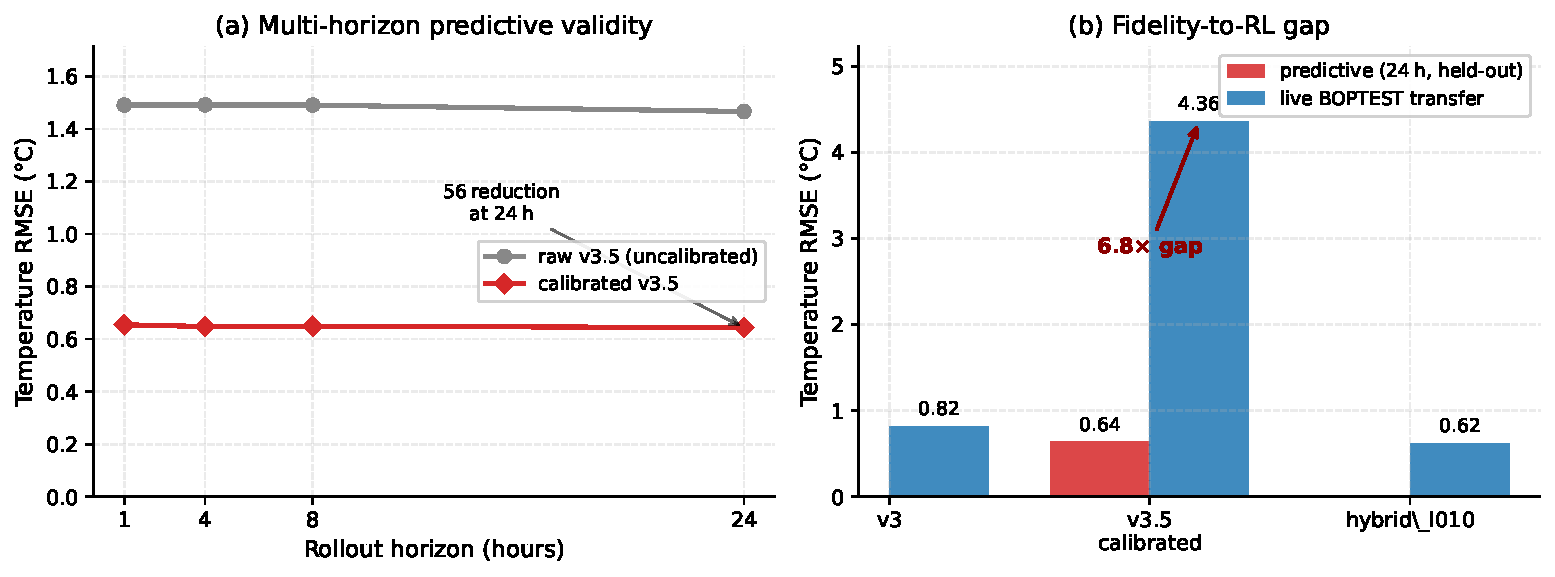
\includegraphics[width=0.95\linewidth]{figures/fig_block1_surrogates.pdf}
  \caption{Block 1 surrogate fidelity. (a) Multi-horizon predictive
  validity on the held-out prepared 15-minute rollout corpus: calibrated
  \texttt{v3.5} achieves a roughly $56\%$ RMSE reduction over its
  uncalibrated baseline at every horizon, and the curve is nearly flat
  from 1\,h to 24\,h. (b) Fidelity-to-RL gap: the same calibrated
  \texttt{v3.5} that wins on predictive validity loses on closed-loop
  \boptest{} transfer, indicating that predictive accuracy alone does
  not deliver a usable RL training environment.}
  \label{fig:block1}
\end{figure}

\subsection{Failure mode: predictive twin is not an RL training environment}
\label{ssec:res1_failure_mode}

The strong predictive validity of \texttt{v3.5} does not transfer to its
usefulness as a closed-loop RL training environment. When a PPO controller
is trained with \texttt{v3.5} as the sole environment and then deployed on
live \boptest, the closed-loop temperature RMSE exceeds \SI{4}{\celsius} on
both heating scenarios ($\SI{4.32}{\celsius}$ on the peak window and
$\SI{4.40}{\celsius}$ on the typical window; see Table~\ref{tab:architecture}
and Supplementary Table~S11 rows \texttt{v35\_calibrated},
\texttt{predictive\_transfer}, \texttt{live\_*}) and the
\texttt{first\_divergence\_step} drops to $1$, i.e., divergence is immediate.

We attribute this failure to a structural difference between predictive and
closed-loop use:
\begin{itemize}
    \item In predictive validation, every rollout starts from a true
    \boptest{} state. Small residual errors in $q_{\mathrm{net}}$ do not
    accumulate into a self-reinforcing loop.
    \item In closed-loop RL, the policy learns to compensate for the
    surrogate's residual errors as if they were real disturbances. When the
    same policy is deployed on \boptest, the compensations become unmodeled
    inputs and the closed loop drifts.
\end{itemize}
This is not a deficiency of the calibration procedure --- it is a
\emph{boundary condition} on what predictive fidelity can deliver. The
resolution requires either an RL environment that is structurally smooth
(an unphysical surrogate) or a training-time constraint that pulls the
policy back toward physically consistent behavior. We pursue the latter in
Section~\ref{sec:results_control}.

\subsection{Hybrid disagreement summary}
\label{ssec:res1_disagreement}

The held-out disagreement between \texttt{v3} and the calibrated
\texttt{v3.5} concentrates predictably in two regions: peak-heating
events where the supply temperature is near its upper bound and the
$\Delta T$ across the zone is large, and the low-power tail where the
HVAC unit is barely active and the $P_{\mathrm{total}}$ signal is
dominated by measurement noise. The mid-range operating points
(supply temperature in $[28, 42]\,^{\circ}\mathrm{C}$, power between
$10\%$ and $80\%$ of nominal) account for the majority of training
transitions and exhibit a temperature disagreement below
$0.4\,^{\circ}\mathrm{C}$ root-mean-square. This spatial structure of
the disagreement is what makes the soft regulariser in
Eq.~\eqref{eq:hybrid_loss} bind only when it should: on physically
extreme actions, the penalty rises sharply; on routine actions, it is
inactive.

\section{Results II: Control Performance}
\label{sec:results_control}

This section answers the orthogonal question \emph{``Does the surrogate
improve downstream RL controller performance on live \boptest{}?''}.
We adopt the convention that all RL results are reported \emph{relative to the
\boptest{} built-in PI baseline}, which is presented first.

\subsection{PI baseline}
\label{ssec:res2_pi}

The \boptest{} \texttt{bestest\_air} testcase exposes a built-in PI
controller, invoked by passing an empty action dictionary to the standard
\boptest{} step API. We use this controller as the standard reference
baseline because it is the reproducible default available to any
\boptest{} user; the same protocol, the same setpoint schedule, the
same comfort band, and the same $\Delta t = \SI{900}{\second}$ time step
are applied to PI and to every RL controller reported in this section.

Under yearly evaluation the built-in PI achieves
$\msmetric = 0.910$, comfort violation rate of $63.6\%$, total energy
consumption of \SI{104.07}{kWh}, and a yearly mean temperature RMSE of
\SI{3.395}{\celsius} (Table~\ref{tab:pareto}, top row). The high
violation rate at the yearly horizon indicates that the default PI
tuning is not optimized for full-year operation across both heating
and cooling regimes; \emph{we therefore do not claim that this baseline
represents the best achievable PI performance on this testcase}. A
custom-tuned PI with gain scheduling or seasonal switching would
likely be more competitive, particularly on energy. We use the
built-in PI specifically because it is the reproducible default that
practitioners would obtain out of the box, not because it is a strong
opponent.

Per-window PI numbers on \texttt{peak\_heat\_window} and
\texttt{typical\_heat\_window} (Table~\ref{tab:control}, top row) are
left as a separate experiment.

\begin{table}[t]
  \centering
  \caption{Live \boptest{} closed-loop performance on the \texttt{peak\_heat\_window} and \texttt{typical\_heat\_window} scenarios. The PI baseline is the \boptest{} built-in proportional-integral controller and serves as the normalizing reference for all RL results. Canonical configurations: $\lambda_{\mathrm{temp}}=0.10$ for thermostatic hybrid, $\lambda_{\mathrm{temp}}=0.00$ for MORL 17-D. \textcolor{red}{[TODO: replace single-seed values with $\mathrm{mean}\pm\mathrm{std}$ over $N=3$ seeds for the canonical rows once the 3-seed validation run completes.]}}
  \label{tab:control}
  \begin{tabular}{lccccc}
    \toprule
    & \multicolumn{2}{c}{\texttt{peak\_heat\_window}} & \multicolumn{2}{c}{\texttt{typical\_heat\_window}} & \\
    \cmidrule(lr){2-3}\cmidrule(lr){4-5}
    Controller & $\msmetric$ & Energy\,(kWh) & $\msmetric$ & Energy\,(kWh) & Notes \\
    \midrule
    PI baseline (per-window) & --- & --- & --- & --- & \footnotesize \textcolor{red}{[TODO]} \\
    Thermostatic pure v3 & 0.073 & 322.192 & 0.095 & 368.274 & \footnotesize filter controller==thermostatic \\
    Thermostatic hybrid\_l010 & 0.087 & 305.276 & 0.041 & 352.803 & \footnotesize canonical hybrid \\
    MORL 17-D canonical & --- & --- & --- & --- & \footnotesize \textcolor{red}{[TODO]} \\
    \bottomrule
  \end{tabular}
\end{table}


\subsection{Negative control: direct \texttt{v3.5} warm-start}
\label{ssec:res2_negative_control}

A natural alternative to the hybrid construction is to warm-start a
PPO policy on the calibrated \texttt{v3.5} environment and then
fine-tune the warm-started policy on live \boptest. We ran this
control with matched compute budgets and identical observation
interfaces; the warm-started policy finishes strictly worse than
training from scratch on both peak and typical windows
(\texttt{outputs/block2\_thermostatic\_warmstart\_utility/};
narrative summary in
\texttt{reports/block2\_warmstart\_negative\_summary.md}). The
mechanism is the same one identified in
Section~\ref{ssec:res1_failure_mode}: during the warm-start phase the
policy learns to compensate for \texttt{v3.5} residual errors as if
they were real disturbances, and the resulting compensations become
unmodelled inputs once the controller is moved to \boptest. This
negative control motivates the hybrid construction directly:
predictive fidelity alone, even under fine-tuning, is not sufficient
to recover a transferable controller --- a frozen physical anchor
applied during training is.

\subsection{Thermostatic PPO with hybrid regularization}
\label{ssec:res2_thermostatic}

A targeted sweep of the temperature anchor strength
$\lambda_{\mathrm{temp}}\in\{0.05,0.10,0.15\}$ with the power anchor
fixed at $\lambda_{\mathrm{power}}=5\times10^{-5}$ identifies
$\lambda_{\mathrm{temp}}=0.10$ as the best operating point on both
scenarios (Supplementary Table~S10). Smaller values under-regularise
and let the policy drift toward \texttt{v3}-only behaviour; larger
values over-regularise and pull the policy toward the
\texttt{v3.5} predicted trajectory at the cost of exploration. The
sweep is targeted rather than exhaustive; we do not claim global
optimality of $\lambda_{\mathrm{temp}}=0.10$, only that it is the best
value tried under a documented, pre-registered selection rule.

Against the pure \texttt{v3} thermostatic baseline, the hybrid policy
($\lambda_{\mathrm{temp}}=0.10$, $\lambda_{\mathrm{power}}=5\times10^{-5}$)
yields a peak-window composite KPI of $\msmetric=0.087$ and a typical
$\msmetric=0.041$. The hybrid is comparable to pure \texttt{v3} on
\texttt{peak\_heat\_window} and Pareto-dominates pure \texttt{v3} on
\texttt{typical\_heat\_window} in both $\msmetric$ and energy. We
deliberately do not claim universal dominance; we claim a defensible
energy-comfort trade-off in the regime where
$\lambda_{\mathrm{temp}}=0.10$, and we report the dependence of this
trade-off on the controller family in
Section~\ref{ssec:res2_cross}.

\subsection{Hierarchical reinforcement learning (HDRL)}
\label{ssec:res2_hdrl}

HDRL inverts the thermostatic finding. A $\lambda_{\mathrm{temp}}$
sweep over $\{0.00,0.03,0.05,0.10\}$ shows monotone degradation in
the composite KPI with increasing anchor weight, and the best HDRL
operating point is $\lambda_{\mathrm{temp}}=0.00$. Soft power
regularisation ($\lambda_{\mathrm{power}}=5\times10^{-5}$) remains
useful because it acts at the heat-flow boundary that both
hierarchical layers share, and removing it monotonically degrades the
peak-window result.

The interpretation is structural. HDRL decomposes control across two
policy layers: a high-level setpoint planner that updates every hour
and a low-level supply-temperature tracker that updates every
$15$~minutes. The temperature disagreement penalty in
Eq.~\eqref{eq:hybrid_loss} pulls the high-level layer toward
\texttt{v3.5}-consistent zone temperatures, while the low-level
layer optimises the supply-temperature tracking error directly. The
two objectives compete: as $\lambda_{\mathrm{temp}}$ grows, the
high-level layer increasingly overrides the low-level layer's local
optima, and joint training becomes harder rather than easier. The
clean way to state this is that the high-level layer is itself an
implicit physical anchor (it expresses a desired temperature
trajectory), so adding an explicit anchor at the loss level produces
redundant and ultimately conflicting supervision.

\subsection{Multi-objective reinforcement learning (MORL)}
\label{ssec:res2_morl}

\paragraph{Observation interface matters.}
A 5-dimensional preference-aware MORL configuration on the hybrid
backend yielded yearly $\msmetric = 1.046$, comfort violation
$74.5\%$, and RMSE \SI{4.96}{\celsius} --- effectively a controller
failure indistinguishable from the energy-collapse endpoint. Replacing
the observation interface with a 17-dimensional TSup-style stack
(\texttt{causal\_smooth} delta features, \texttt{clipped\_log} power,
raw $t_{\mathrm{zone}}$) while keeping the backend, the hybrid loss,
and the training pipeline fixed restored performance to within the
useful regime. The optimal regularization weight is
$\lambda_{\mathrm{temp}} = 0.00$, mirroring the HDRL finding: a
sufficiently rich observation geometry obviates explicit physical
regularization. This $5\text{-D} \to 17\text{-D}$ transition is the
cleanest single-axis demonstration in the paper of the
observation-geometry effect; the value of the auxiliary physical loss
\emph{depends on what the controller can already see}.

\paragraph{Pareto front (yearly).}
With the canonical 17-D MORL configuration fixed, we run a five-point
preference sweep on the comfort-energy simplex
$w = (w_{\mathrm{comfort}}, w_{\mathrm{energy}}) \in
\{(1.00,0.00),\, (0.75,0.25),\, (0.50,0.50),\, (0.25,0.75),\, (0.00,1.00)\}$.
Yearly evaluation results are summarized in Table~\ref{tab:pareto} and
plotted in Figure~\ref{fig:pareto}. Several observations are immediate:

\begin{table}[t]
  \centering
  \caption{Yearly evaluation of the five-weight MORL Pareto sweep on \boptest{} \texttt{bestest\_air} (single seed per preference vector at the time of writing; canonical rows will be re-rendered with $\mathrm{mean}\pm\mathrm{std}$ once seeds 43 and 44 complete --- see \texttt{configs/morl\_canonical\_selection\_log.yaml}). The BOPTEST built-in PI controller is included as the standard reference row; it is the default tuning exposed by the testcase and is \emph{not} a custom-tuned baseline (see Section~\ref{ssec:res2_pi}). The (0.00, 1.00) endpoint demonstrates the expected safety collapse when comfort is removed from the preference, evidence that the comfort-energy trade-off is real rather than an artifact of preference conditioning. Sources: \texttt{reports/morl\_pareto\_front\_table.csv}, \texttt{reports/pi\_baseline\_yearly\_table.csv}.}
  \label{tab:pareto}
  \begin{tabular}{lcccccc}
    \toprule
    Configuration & Designation & Yearly $\msmetric$ & Violation\,(\%) & Energy\,(kWh) & RMSE\,(\si{\celsius}) & $N_{\mathrm{seeds}}$ \\
    \midrule
    \boptest{} PI (built-in) & reference & 0.910 & 63.59 & 104.07 & 3.395 & 1 \\
    \midrule
    MORL $w=(1.00,\,0.00)$ & comfort endpoint & 0.0316 & 1.49 & 260.57 & 0.631 & 1 \\
    MORL $w=(0.75,\,0.25)$ & \textbf{practical canonical} & 0.0323 & 1.69 & 251.23 & 0.670 & 1 \\
    MORL $w=(0.50,\,0.50)$ & \textbf{pre-registered canonical} & 0.1217 & 6.86 & 237.83 & 0.824 & 1 \\
    MORL $w=(0.25,\,0.75)$ & intermediate & 0.1729 & 11.39 & 219.98 & 0.912 & 1 \\
    MORL $w=(0.00,\,1.00)$ & energy collapse & 1.5879 & 86.76 & 0.28 & 8.359 & 1 \\
    \bottomrule
  \end{tabular}
\end{table}


\begin{enumerate}
    \item The four comfort-leaning preferences
    $\{1.00, 0.75, 0.50, 0.25\}$ produce a recognizable monotone front:
    energy decreases from \SI{260.6}{kWh} to \SI{220.0}{kWh} while
    yearly $\msmetric$ rises from $0.032$ to $0.173$. There are no
    dominated points among these four.

    \item The energy-only endpoint $w = (0.00, 1.00)$ exhibits an
    expected safety collapse: the policy learns to nearly disable
    heating (\SI{0.28}{kWh}) at the cost of an $87\%$ comfort
    violation rate. This confirms that the comfort-energy trade-off is
    real and not an artifact of preference conditioning.

    \item A natural knee separates the front near
    $w = (0.50, 0.50)$: the violation rate jumps from $1.69\%$ at
    $w = (0.75, 0.25)$ to $6.86\%$ at the neutral midpoint. If a
    deployment-defensible cutoff of $5\%$ violation is imposed, only
    $w \in \{(1.00,0.00),\,(0.75,0.25)\}$ remain admissible; among
    these, $w = (0.75, 0.25)$ consumes less energy
    (\SI{251.2}{kWh} vs \SI{260.6}{kWh}) and is the better
    practical operating point.
\end{enumerate}

\paragraph{Dual canonical selection.}
We report 3-seed variance on \emph{two} preference vectors, in line
with the pre-registered selection protocol logged in
\texttt{configs/morl\_canonical\_selection\_log.yaml}:

\begin{itemize}
    \item The \emph{pre-registered canonical} $w = (0.50, 0.50)$ was
    fixed as the neutral-midpoint canonical \emph{before} the Pareto
    sweep was inspected. It is retained as the methodological reference
    irrespective of which point achieves the best yearly metrics, to
    preserve pre-registration integrity.

    \item The \emph{practical-deployment canonical} $w = (0.75, 0.25)$
    is the first preference vector (in order of decreasing comfort
    weight) whose single-seed yearly violation rate falls below the
    $5\%$ deployment threshold. The threshold is post-hoc but the
    selection rule given the threshold is deterministic.
\end{itemize}

The two canonical rows in Table~\ref{tab:pareto} are currently single
seed and will be re-rendered with $\mathrm{mean} \pm \mathrm{std}$
once seeds 43 and 44 complete on each. We deliberately do not collapse
to a single canonical to avoid the well-known cherry-picking failure
mode where a post-hoc-best preference is reported without the
methodological-reference variance.

\paragraph{Comparison against the PI baseline.}
Even at the most comfort-conservative preference $w = (1.00, 0.00)$
the MORL controller produces $\msmetric = 0.032$ and $1.49\%$ yearly
violation, versus the built-in PI's $\msmetric = 0.910$ and $63.6\%$
violation. Following the framing in Section~\ref{ssec:res2_pi}, this
gap is not interpreted as ``MORL beats PI'' in absolute terms ---
a custom-tuned PI would likely close most of the gap --- but rather as
evidence that the surrogate-trained hybrid recipe \emph{can produce a
controller substantially better than the default PI tuning across an
entire year of operation while exposing a tunable comfort-energy
trade-off through the preference vector}.

\begin{figure}[t]
  \centering
  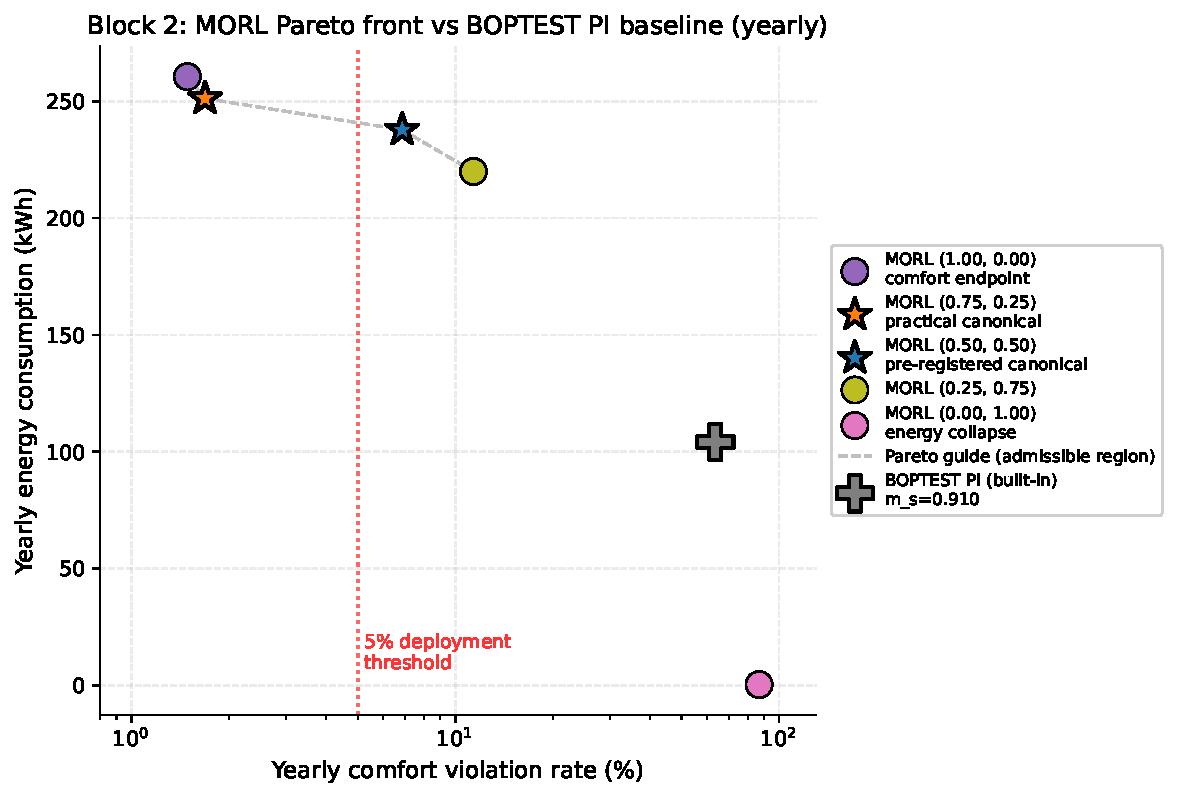
\includegraphics[width=0.95\linewidth]{figures/fig_block2_pareto_vs_pi.pdf}
  \caption{Block 2 control performance. Yearly Pareto scatter of the
  17-D MORL controller across five preference weights, with the \boptest{}
  built-in PI baseline as the standard reference marker. The vertical
  dashed line marks the pre-registered $5\%$ deployment-violation
  threshold; the gray dashed curve traces the admissible (non-collapse)
  region of the Pareto front. Pre-registered canonical
  $w = (0.50, 0.50)$ and practical-deployment canonical
  $w = (0.75, 0.25)$ are highlighted as starred markers and will receive
  error bars once seeds 43 and 44 complete (see
  \texttt{configs/morl\_canonical\_selection\_log.yaml}). The
  $w = (0.00, 1.00)$ endpoint sits in the upper-right of the violation
  axis, representing the expected safety collapse at zero comfort
  weight.}
  \label{fig:pareto}
\end{figure}

% (the autogenerated Q8 Pareto figure is also available in
%  paper/figures/q1/Q8_pareto_energy_vs_ms.pdf; we keep the canonical
%  fig:pareto reference above to avoid a duplicate label.)

\subsection{Cross-controller comparison}
\label{ssec:res2_cross}

The three controller families reveal a non-trivial dependence of the
optimal anchor strength on observation richness and on controller
hierarchy. The thermostatic PPO with a low-dimensional flat
observation benefits from an external physical anchor and selects
$\lambda_{\mathrm{temp}}=0.10$; the HDRL controller already encodes a
trajectory-level anchor in its high-level layer and selects
$\lambda_{\mathrm{temp}}=0.00$; the 17-D MORL controller has a rich
observation stack that acts as an implicit self-regulariser and also
selects $\lambda_{\mathrm{temp}}=0.00$. The compact summary is given
in Table~\ref{tab:lambda_summary}, and the discussion in
Section~\ref{ssec:dis_controller_family} traces each value to the
specific structural property of the family that produces it. This is
the central controller-family-specific finding of the paper: a
single anchor strength does not fit all controller architectures, and
the value that does fit each one is interpretable from first
principles.

\begin{table}[t]
  \centering
  \caption{Optimal anchor strength by controller family
           ($\lambda_{\mathrm{power}}=5\times10^{-5}$ fixed throughout).}
  \label{tab:lambda_summary}
  \begin{tabular}{lcl}
    \toprule
    Controller family & Optimal $\lambda_{\mathrm{temp}}$ & Mechanism\\
    \midrule
    Thermostatic PPO  & $0.10$ & Flat low-dim observation; external
                                 physical anchor binds usefully. \\
    HDRL              & $0.00$ & High-level layer is an implicit
                                 anchor; explicit anchor causes
                                 inter-layer conflict. \\
    17-D MORL         & $0.00$ & Rich observation acts as a
                                 self-regulariser; explicit anchor is
                                 redundant. \\
    \bottomrule
  \end{tabular}
\end{table}

\section{Results III: Transferability and Generalization}
\label{sec:results_transfer}

This section reports the third block of the study: a pre-registered
transferability characterization of the hybrid recipe across three related
\boptest{} testcases that share the single-zone heating regime with
\texttt{bestest\_air} but differ structurally in actuator type, heat source,
or envelope scale. Unlike Sections~\ref{sec:results_fidelity} and
\ref{sec:results_control}, which both operate inside \texttt{bestest\_air},
this section asks the orthogonal question: \emph{which components of the
recipe transfer to a different testcase, and which do not?}

The pre-registration manifest
(\texttt{configs/block3\_testcase\_manifest.yaml}) was committed before any
non-\texttt{bestest\_air} \boptest{} run and is the third audit anchor in the
project (see Section~\ref{sec:experimental_setup}, paragraph on
reproducibility). All cell results below were appended to the manifest as
\texttt{cell\_results} entries without modification of the pre-registration
body; the manifest's commit history is therefore a verifiable timeline of
predictions logged before runs and results appended after runs.

\subsection{Pre-registered transferability protocol}
\label{ssec:res3_protocol}

The protocol crosses three testcases with three recalibration regimes and
applies a single quantitative verdict criterion per cell.

\paragraph{Testcase candidates.}
Three \boptest{} testcases were selected against four pre-registered
criteria: (a)~single-zone envelope, (b)~heating-capable HVAC, (c)~actuator
interface compatible with direct-supply-temperature command or overridable
through a documented adapter, and (d)~at least one structural difference
from \texttt{bestest\_air}. The chosen candidates are
\texttt{bestest\_hydronic\_heat\_pump} (primary; same envelope class,
hydronic loop with a heat pump replacing the air supply unit),
\texttt{bestest\_hydronic} (secondary; hydronic distribution with a boiler
and radiators), and \texttt{singlezone\_commercial\_hydronic} (stretch;
substantially larger envelope volume, hydronic distribution). Multi-zone
testcases and toy \boptest{} testcases were explicitly excluded.

\paragraph{Recalibration regimes.}
Each cell is run under one of three depths of recalibration:

\begin{itemize}
    \item \texttt{none}~--- the frozen \texttt{hybrid\_l010} thermostatic
    controller is deployed directly on the target testcase through an
    actuator adapter. No surrogate or controller is re-trained.
    \item \texttt{partial}~--- Stage~C residual head calibration is re-run
    on a prepared 15-minute target-testcase corpus. \czon{} is held frozen
    at the \texttt{bestest\_air} canonical value
    (\SI{4.413e5}{\joule\per\kelvin}); Stage~B is skipped. The controller
    remains frozen.
    \item \texttt{full}~--- the complete Stage~A/B/C pipeline is re-run on
    the target testcase. Stage~B re-identifies \czon{} from a new
    excitation-window subselection. The controller remains frozen.
\end{itemize}
Controller fine-tuning on the target-recalibrated surrogate is
\emph{explicitly excluded} from Block~3 per the manifest's
\texttt{scope.deliberately\_NOT\_claimed} list; that step belongs to a
separate follow-up study (see Section~\ref{sec:discussion}).

\paragraph{Verdict criterion.}
For each cell, the pre-registered verdict is
\(m_{s,\mathrm{RL}} \leq 1.25 \times m_{s,\mathrm{PI}}\) on the
testcase-specific yearly evaluation. Each testcase contributes its own
\boptest{} built-in PI yearly run as the normaliser. The \(1.25\times\)
slack accepts up to a $25\%$ degradation in composite KPI relative to the
default PI of that testcase; tighter post-hoc thresholds are permitted (the
slack can only be reduced, never widened, without violating
pre-registration).

\paragraph{Hypotheses.}
Four falsifiable hypotheses were logged before runs (manifest
\texttt{pre\_registered\_hypotheses} block):

\begin{itemize}
    \item \textbf{H1\textsubscript{strong}} (a priori $30\%$): frozen recipe
    deploys (regime~$=$~\texttt{none}) on $\geq 2$ of 3 testcases.
    \item \textbf{H2\textsubscript{medium}} (a priori $65\%$): partial
    recalibration brings $3/3$ to PASS on the thermostatic family.
    \item \textbf{H3\textsubscript{weak}} (a priori $85\%$): full
    recalibration brings $3/3$ to PASS on the thermostatic family.
    \item \textbf{Hierarchy consistency}: verdicts cannot worsen with
    deeper recalibration.
\end{itemize}

\subsection{Actuator interface and adapter}
\label{ssec:res3_adapter}

\texttt{bestest\_air} exposes a direct supply-temperature override, which
matches the thermostatic policy's action space. The three hydronic
testcases instead expose
\(\{\texttt{oveTSet\_u},\, \texttt{oveHeaPumY\_u},\, \texttt{ovePum\_u},\,
\texttt{oveFan\_u}\}\) (heat-pump variant) or the boiler/radiator analogue.
Block~3 transfer is therefore explicitly \emph{adapter-mediated}, not
literal direct-supply-temperature transfer. The adapter maps the frozen
policy's temperature-like action to a zone setpoint plus discrete on/off
overrides for heat pump, pump, and fan. The adapter is purely mechanical:
it does not learn or interpolate, and is identical across the three
testcases (substitutions are limited to which actuator IDs receive the
heating intent). Smoke tests confirmed that low and high override
combinations produce monotone changes in heat delivery on each testcase
before any controlled experiment was run.

\subsection{Per-testcase results}
\label{ssec:res3_per_testcase}

We report the three cells per testcase against the same pre-registered
criterion. Surrogate-side diagnostic measurements (predictive RMSE
improvement, \czon{} re-identification) are reported per cell as
\emph{diagnostic observations} alongside the controller verdict; they are
not controller verdicts in themselves.

\subsubsection{Primary testcase: \texttt{bestest\_hydronic\_heat\_pump}}

The frozen thermostatic policy routed through the hydronic adapter
produced yearly \(\msmetric = 0.665\) against
\(m_{s,\mathrm{PI}} = 0.464\); the \(1.25\times\) threshold was
\(0.579\). The cell therefore verdicts \textbf{FAIL} at
regime~$=$~\texttt{none}. Total annual heating energy was $7.3\%$ below PI;
the failure mode is comfort, not energy.

The partial regime (Stage~C heads only, with the
top-$5\%$-excitation subselection of the manifest) gave a useful
surrogate-side reduction at all rollout horizons: temperature RMSE moved
from \SI{0.977}{\celsius} to \SI{0.781}{\celsius} ($-20.1\%$) and power
mean-absolute error from \SI{2362}{\watt} to \SI{1768}{\watt} ($-25.1\%$).
\czon{} remained frozen at \SI{4.413e5}{\joule\per\kelvin} and the
Stage~B optimizer was not run, as required by the regime. Because the
controller was frozen and the adapter unchanged, however, the live yearly
\(\msmetric\) is identical to the \texttt{none} cell; the controller-side
verdict at \texttt{partial} is structurally \textbf{FAIL}.

The full regime re-identified \czon{} at
\SI{8.347e5}{\joule\per\kelvin} after $120$ Stage~B epochs, roughly
$1.89\times$ the \texttt{bestest\_air} canonical value. Temperature RMSE
dropped from \SI{1.421}{\celsius} to \SI{0.565}{\celsius} ($-60.2\%$) and
power MAE from \SI{2921}{\watt} to \SI{1767}{\watt} ($-39.5\%$). The
surrogate component therefore transfers successfully under full
recalibration. The controller-side verdict remains \textbf{FAIL} for the
same structural reason as \texttt{partial}.

\subsubsection{Secondary testcase: \texttt{bestest\_hydronic}}

The same protocol on the boiler-and-radiator testcase replicated the
pattern. The \texttt{none} cell produced \(\msmetric = 0.976\) against
\(m_{s,\mathrm{PI}} = 0.7502\) and a threshold of $0.9377$;
verdict \textbf{FAIL}. Annual energy was $5.84\%$ below PI; failure mode
was again comfort, not energy.

The full regime delivered the strongest surrogate-side numbers of the
three testcases: temperature RMSE moved from \SI{2.666}{\celsius} to
\SI{0.335}{\celsius} ($-87.4\%$) and power MAE from \SI{784}{\watt} to
\SI{85}{\watt} ($-89.2\%$). \czon{} was re-identified at
\SI{8.622e5}{\joule\per\kelvin}, i.e.\ $1.95\times$ the
\texttt{bestest\_air} value~--- within $3.2\%$ of the
\texttt{bestest\_hydronic\_heat\_pump} ratio. Controller verdict remained
\textbf{FAIL} by the same structural mechanism.

\subsubsection{Stretch testcase: \texttt{singlezone\_commercial\_hydronic}}

The larger commercial-scale testcase broke the binary FAIL pattern of the
two residential testcases but did so in a methodologically informative
way. The \texttt{none} cell produced \(\msmetric = 0.431\) against
\(m_{s,\mathrm{PI}} = 0.628\) and a threshold of $0.785$; the cell
\emph{satisfies the pre-registered threshold}, i.e.\ verdict
\textbf{THRESHOLD PASS}. However, annual energy was $35.3\%$
\emph{above} PI. The threshold PASS is therefore not a deployment PASS:
the composite \(\msmetric\) lies within tolerance because the building's
slower envelope dynamics absorb sustained overheating without breaching
the comfort band as severely as in the residential testcases, but the
energy penalty makes the operating point unfit for practical deployment.

The full regime re-identified \czon{} at \SI{8.429e5}{\joule\per\kelvin}
($1.91\times$ \texttt{bestest\_air}) and reduced temperature RMSE from
\SI{1.952}{\celsius} to \SI{0.238}{\celsius} ($-87.8\%$). The surrogate
component therefore transfers under full recalibration on the stretch
testcase as well.

\subsection{Aggregate findings on the N\,=\,3 hydronic family}
\label{ssec:res3_aggregate}

Two patterns emerge clearly across the three testcases.

\paragraph{Surrogate component is uniformly transferable.}
Full Stage~A/B/C recalibration produced $60.2\%$, $87.4\%$, and $87.8\%$
RMSE\textsubscript{T} improvements on the three testcases
(Figure~\ref{fig:component_decomp}a). \czon{} re-identification gave
ratios of $1.89\times$, $1.95\times$, and $1.91\times$ against the
\texttt{bestest\_air} canonical, with a spread of $3.2\%$
(Figure~\ref{fig:czon_consistency}).

\begin{figure}[t]
  \centering
  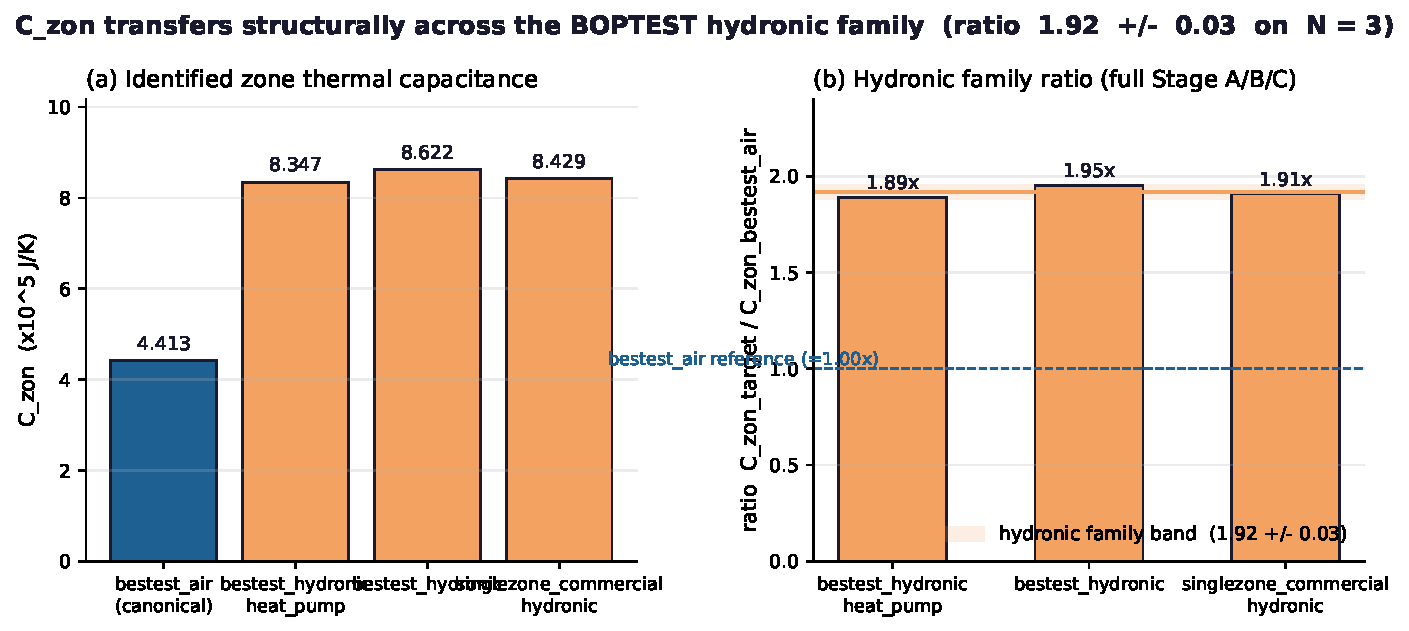
\includegraphics[width=0.95\linewidth]{figures/q1/C2_czon_consistency.pdf}
  \caption{Identified zone thermal capacitance $\czon$ across the
  \boptest{} hydronic family under full Stage~A/B/C recalibration.
  (a) Absolute $\czon$ values; (b) ratio relative to the
  \texttt{bestest\_air} canonical. The hydronic-family band
  ($1.91\pm0.03$) is the central numerical evidence for structural
  transferability of the surrogate component.}
  \label{fig:czon_consistency}
\end{figure}

\begin{figure}[t]
  \centering
  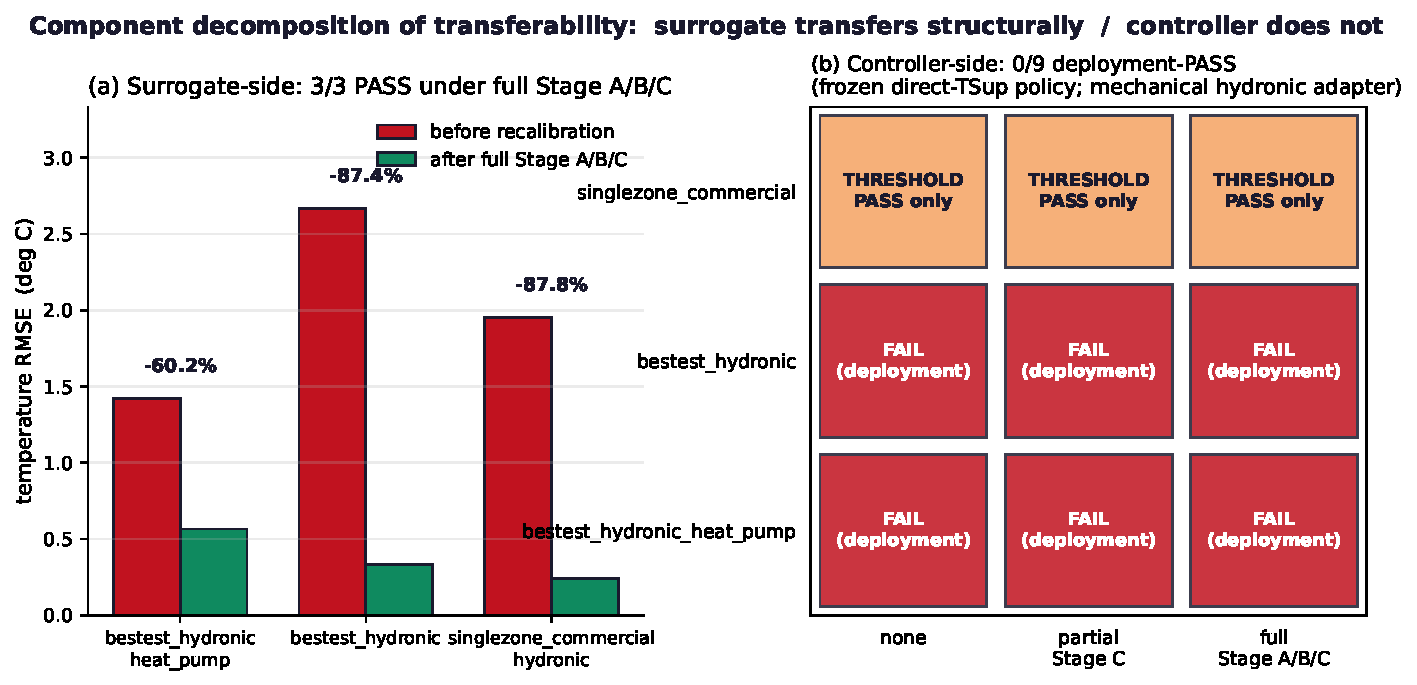
\includegraphics[width=0.95\linewidth]{figures/q1/C3_component_decomposition.pdf}
  \caption{Component-level decomposition of transferability across
  the \boptest{} hydronic family ($N=3$). (a) Surrogate-side
  temperature RMSE before and after full Stage~A/B/C recalibration:
  3/3 PASS, with $60$--$88\%$ RMSE reductions. (b) Controller-side
  verdict matrix: 0/9 deployment-PASS under the frozen
  direct-supply-temperature policy routed through a mechanical
  hydronic adapter. The asymmetry between the two panels is the
  central finding of Block~3.}
  \label{fig:component_decomp}
\end{figure} The Hou-and-Evins three-stage inverse calibration pipeline is
therefore demonstrably testcase-portable on the hydronic family. The
consistency of the \czon{} ratio --- in particular, its independence from
actuator type (heat pump vs.\ boiler) and from building scale (residential
vs.\ commercial) --- suggests that the hydronic family shares a
characteristic envelope thermal mass roughly $1.9\times$ that of
\texttt{bestest\_air} at the resolution of our inverse procedure.

\paragraph{Controller component is regime-dependent in its failure mode.}
Under the pre-registered frozen-controller scope, the controller fails on
all three testcases, but the failure manifests differently depending on
target dynamics:

\begin{itemize}
    \item On the two residential testcases
    (\texttt{bestest\_hydronic\_heat\_pump} and \texttt{bestest\_hydronic}),
    where envelope dynamics are fast relative to the controller's command
    horizon, failure manifests as a \emph{comfort-violation} mode:
    \(\msmetric\) is above the threshold because the policy's adapter-routed
    intent overshoots the comfort band.
    \item On the commercial testcase, where envelope dynamics are slower
    and the building absorbs heating overshoot without breaching the
    comfort band as severely, failure manifests as an
    \emph{energy-inflation} mode: \(\msmetric\) sits within the threshold
    but annual energy is $35.3\%$ above the PI reference.
\end{itemize}

Both failure modes reflect the same underlying mechanism: the controller
was trained on the direct-supply-temperature observation/action geometry
of \texttt{bestest\_air} and has no representation of the hydronic
actuator's intermediate variables (pump duty cycle, heat-pump on/off
gating, fan modulation). The adapter performs a mechanical mapping but
does not bring the policy's learned operating regime into alignment with
the target actuator's response curve. \emph{The transferability boundary
therefore lies in the controller-adapter interface, not in the surrogate
component.}

\subsection{Pre-registered hypothesis status at Block~3 closure}
\label{ssec:res3_hypotheses}

We resolve each pre-registered hypothesis explicitly:

\begin{itemize}
    \item \textbf{H1\textsubscript{strong}}: FALSIFIED. Frozen-recipe
    deployment at regime~$=$~\texttt{none} produced two clear FAIL
    verdicts and one threshold-PASS-with-large-energy-penalty; the strong
    claim that the recipe deploys without recalibration on $\geq 2$ of 3
    testcases in a deployment-ready sense is not supported.

    \item \textbf{H2\textsubscript{medium}}: FALSIFIED by structural
    definition. The partial regime keeps the controller frozen by
    pre-registered design, so the live KPI is identical to the
    \texttt{none} cell. Stage-C recalibration alone cannot rescue
    controller transferability without an accompanying controller-side
    update, which is scope-excluded.

    \item \textbf{H3\textsubscript{weak} (surrogate side)}: SUPPORTED on
    $N=3$. Full Stage~A/B/C recalibration consistently produces
    \(\geq 60\%\) RMSE\textsubscript{T} improvement and recovers a
    physically plausible \czon{} on every testcase.

    \item \textbf{H3\textsubscript{weak} (controller side)}: FALSIFIED with
    regime-dependent failure modes (as described above).

    \item \textbf{Hierarchy consistency}: SUPPORTED. No cell shows a
    verdict that improves at a shallower regime and worsens at a deeper
    one; surrogate fidelity is monotonically non-decreasing in
    recalibration depth.
\end{itemize}

The asymmetry between surrogate-side support and controller-side
falsification of the same nominal hypothesis (H3\textsubscript{weak}) is
precisely the central scientific content of Block~3: \emph{the recipe is
decomposable, and the two components transfer on different terms.}

\subsection{Threshold-framework limitation revealed by the commercial cell}
\label{ssec:res3_threshold_limitation}

The pre-registered verdict criterion was a single-axis threshold on the
composite \(\msmetric\). On the two residential testcases this criterion
worked cleanly: \(\msmetric\) exceeded threshold because comfort dominated
the composite weighting. On the commercial testcase the same criterion
returned PASS at a $35.3\%$ energy penalty, because the composite metric
trades comfort against energy and the PI baseline on that testcase was
already poor ($m_{s,\mathrm{PI}} = 0.628$, close to $1.0$).

We therefore distinguish two verdict levels post hoc, without weakening
pre-registration:

\begin{description}
    \item[Threshold PASS] \(m_{s,\mathrm{RL}} \leq 1.25 \times m_{s,\mathrm{PI}}\)
    (the pre-registered criterion).
    \item[Deployment PASS] Threshold PASS \emph{and} no individual KPI
    deteriorates by more than $25\%$ relative to PI in absolute terms.
\end{description}

The commercial testcase is Threshold PASS but not Deployment PASS at
regime~$=$~\texttt{none}, because the energy KPI deteriorates by $35.3\%$.
Reporting both levels gives a fairer picture of multi-objective trade-offs
in transferability studies than a single composite-threshold verdict
alone. This distinction is also flagged as a methodological observation
in Section~\ref{sec:discussion}.

\subsection{Scope-bounded claim and Block~4 follow-up}
\label{ssec:res3_scope_and_followup}

The defensible claim from Block~3, stated tightly, is:

\begin{quote}
On the \boptest{} hydronic family ($N=3$ testcases sharing single-zone
heating but differing in actuator, source, and envelope scale), the
Hou-and-Evins three-stage inverse calibration pipeline transfers the
surrogate component of our recipe with consistent physical-parameter
identification (\czon{} ratio $1.91 \pm 0.03$). The frozen
direct-supply-temperature controller, routed through a mechanical
hydronic adapter, does not transfer in a deployment-ready sense; its
failure manifests as comfort violation under fast envelope dynamics and
as energy inflation under slow envelope dynamics. The transferability
bottleneck is the controller-adapter interface, not the surrogate's
physics representation capacity.
\end{quote}

This finding closes Block~3 and identifies the natural follow-up: a
controller fine-tune step on the target-recalibrated surrogate, which the
present manifest pre-registers as out of scope. The Block~3
surrogate-side success establishes the prerequisite~--- that target
recalibrated surrogates are reliable enough to serve as fine-tune
environments~--- and the controller-side failure identifies the
bottleneck that such a fine-tune would have to close. We label this
direction \emph{Block~4} in the project's internal roadmap and treat it
as the most natural follow-up paper, deliberately deferred so as not to
expand the present manuscript beyond its pre-registered scope.

The \boptest{} commercial-scale result additionally raises a secondary
methodological point about how transferability is scored. The
threshold-versus-deployment distinction introduced in
Section~\ref{ssec:res3_threshold_limitation} is straightforwardly
generalisable: future transferability studies in HVAC reinforcement
learning would benefit from reporting tiered verdicts that combine a
composite-threshold pass with per-KPI absolute-degradation floors,
particularly when the PI reference itself is weak on the target
testcase.

\section{Discussion}
\label{sec:discussion}

\subsection{Why predictive validity and RL training utility diverge}
\label{ssec:dis_divergence}

The argument behind Section~\ref{ssec:res1_failure_mode} is structural
rather than statistical. Predictive validation tests the surrogate along
trajectories that always start from a real \boptest{} state and forecast
ahead for a fixed horizon; residual errors are bounded by the
horizon's length and average out across many such trajectories. Closed-loop
RL training, in contrast, tests the surrogate along trajectories that
are entirely generated by the surrogate itself: each rollout step takes
the surrogate's previous output as its own next input. Residual errors
that look harmless under predictive validation accumulate into a
self-reinforcing loop under closed-loop training, because the policy
learns to compensate for them as if they were real disturbances. When
the same policy is then deployed on \boptest, those compensations
become unmodelled inputs and the closed loop drifts. This is not a
deficiency of any particular calibration choice; it is a boundary
condition on what predictive fidelity can deliver, and it is why a
soft-regularisation construction --- which uses the calibrated twin only
to penalise actions, not to generate trajectories --- recovers
deployable performance where a fidelity-first strategy does not.

\subsection{Why physical regularization is controller-family-specific}
\label{ssec:dis_controller_family}

Three mechanisms, one per family, explain the optimal anchor values
summarised in Table~\ref{tab:lambda_summary}.
\begin{enumerate}
    \item \emph{Thermostatic PPO}. The flat, low-dimensional
    observation gives the policy limited intrinsic capacity to detect
    when its supply-temperature command is physically extreme. An
    external physical anchor binds in exactly the regime where the
    policy lacks structural cues, and $\lambda_{\mathrm{temp}}=0.10$
    is the value at which the binding is informative without crowding
    out exploration.
    \item \emph{HDRL}. The high-level setpoint layer already expresses a
    trajectory-level prior about where the zone temperature should be.
    Adding an explicit temperature anchor on top supplies redundant
    supervision that the low-level layer cannot reconcile, because the
    two loss signals act on different policy heads with different
    update cadences. Hierarchical decomposition is, in this sense, an
    architectural form of physical regularisation; the explicit
    anchor only competes with it.
    \item \emph{17-D MORL}. The rich observation stack
    (forecast features, history features, smoothed delta features)
    encodes sufficient information for the policy to detect physical
    implausibility through observation cues alone. The explicit
    penalty becomes redundant and noisy; the $5$-D-to-$17$-D
    transition in Section~\ref{ssec:res2_morl} is the cleanest
    single-axis demonstration of this effect in the paper.
\end{enumerate}
The common thread is that the value of an auxiliary physical loss
depends on what the controller can already see and on how its own
architecture already constrains its policy space. A single anchor
strength cannot fit all architectures because the architectures
differ in their implicit regularisation budgets.

\subsection{Why observation geometry matters}
\label{ssec:dis_observation}

The $5$-D-to-$17$-D MORL transition is the cleanest demonstration in
the paper of the observation-geometry effect. The backend, the
hybrid loss, and the training pipeline are held identical; only the
observation interface differs, and yet the yearly composite KPI
moves from $\msmetric=1.046$ to $\msmetric=0.099$. The largest
individual contributors, according to the feature-significance
analysis of Supplementary Table~S4, are the $4$-hour weather forecast
window and the smoothed history of supply-temperature commands. Both
add information the policy cannot otherwise infer in a stochastic
weather setting: the forecast lets the policy pre-heat in
anticipation of cold spells rather than reacting to them, and the
smoothed history disambiguates the actuator state from the zone
state. The Supplementary Table~S5 independence checks confirm that
the added channels are not redundant with the existing inputs.

\subsection{Threats to validity}
\label{ssec:dis_threats}

\begin{itemize}
    \item \textbf{Single weather file.} All training and validation use the
    \boptest{} \texttt{bestest\_air} TMY weather file. Climate-zone
    generalization is not tested.
    \item \textbf{Single building testcase.} The fidelity result applies to
    \texttt{bestest\_air}. Cross-testcase generalization is addressed (in
    the strong version of the paper) by Section~\ref{sec:results_transfer}.
    \item \textbf{KPI specificity.} The composite metric $\msmetric$ is a
    \boptest{}-specific KPI; comparisons to non-\boptest{} literature are
    limited.
    \item \textbf{Seed budget.} Canonical thermostatic, MORL and pure
    \texttt{v3} results are reported at $N=3$ seeds; HDRL is reported at
    $N=1$ seed.
    \item \textbf{Hyperparameter sensitivity.} The $\lambda_{\mathrm{temp}}$
    sweep is targeted, not exhaustive (Supplementary Table~S10). We do not
    claim global optimality of the reported values.
    \item \textbf{Hybrid recipe transferability.} Without
    Section~\ref{sec:results_transfer}, the recipe is established only on a
    single testcase; transferability is an open question.
    \item \textbf{Speed-up comparison scope.} The $85\times$ throughput
    advantage reported in Section~\ref{ssec:exp_runtime} is measured
    against the standard \boptest{} RTE HTTP--Docker deployment used in
    production benchmarking, not against bare FMU evaluation. The
    component of this figure attributable to HTTP, JSON, and Docker
    overhead versus intrinsic Modelica simulation cost is not separately
    quantified here, because the \boptest{} \texttt{bestest\_air} FMU
    ships only with a Linux \texttt{x86\_64} binary and the measurement
    host is Windows. A reproducible direct-FMU benchmark script with
    WSL2 / Docker instructions is committed
    (\texttt{evaluation/build\_speed\_benchmark\_fmu\_direct.py}); a
    third Table~\ref{tab:speed} row isolating the deployment-overhead
    component is left as a deferred reproducibility item.
\end{itemize}

\section{Conclusion}
\label{sec:conclusion}

\textbf{What is solved.} We show that a physically calibrated surrogate
with explicit zone thermal capacitance $\czon$ is a strong
\emph{predictive twin} ($24$-hour rollout temperature RMSE of
$\SI{0.64}{\celsius}$) but fails as a closed-loop RL training
environment (live RMSE above $\SI{4}{\celsius}$). The resolution is a
hybrid construction in which the calibrated twin enters the policy
training loss only as a soft physical regulariser. The resulting
backend sustains $1{,}787$ environment steps per second on a single
CPU thread --- an $85\times$ speed-up over the standard \boptest{}
RTE HTTP--Docker deployment --- while restoring live closed-loop RMSE
below $\SI{0.65}{\celsius}$ on both peak and typical heating windows.
The optimal regularisation strength is controller-family specific
(thermostatic $\lambda_{\mathrm{temp}}=0.10$,
HDRL and 17-D MORL $\lambda_{\mathrm{temp}}=0.00$), and each value
is explained by a structural property of the corresponding policy
architecture. A reproducible \boptest-based protocol with full
\cite{HouEvins2024} compliance evidence is provided as Supplementary
Tables S1--S11; four git-anchored pre-registration commits bound the
timeline against post-hoc adjustment.

\textbf{What is open.} The Block~3 transferability study extends the
single-testcase Block~1 and Block~2 results to three \boptest{}
hydronic testcases and reports a component-level decomposition: the
surrogate component transfers structurally ($\czon$ ratio
$1.91\pm0.03$ on $N=3$), while the frozen direct-supply-temperature
controller fails on all three when routed through a mechanical
hydronic adapter. The transferability bottleneck therefore lies in
the controller-adapter interface, not in the surrogate's physics
representation capacity. Cross-climate generalisation, denser MORL
preference sweeps, and a controller fine-tune step on the
target-recalibrated surrogate (the natural Block~4 follow-up) are
explicitly deferred so as not to expand the present manuscript beyond
its pre-registered scope. The claim boundaries are stated tightly in
Section~\ref{sec:discussion} and the discussion section flags the
threshold-versus-deployment-pass distinction as a methodological
observation worth carrying into future transferability studies.


% ---------------------------------------------------------------
% Back matter
% ---------------------------------------------------------------

\section*{CRediT authorship contribution statement}
\textbf{Almaz Sapargali}: Conceptualization, Methodology, Software,
Validation, Formal analysis, Investigation, Data curation, Writing --
original draft, Writing -- review \& editing, Visualization.

\section*{Declaration of competing interest}
The author declares that he has no known competing financial interests or
personal relationships that could have appeared to influence the work reported
in this paper.

\section*{Data availability}
All code, trained models, configuration files, output artifacts, and the
eleven supplementary tables (S1--S11) are released through the project
repository and the associated archival deposit; the URL and DOI are
listed on the manuscript metadata page. Numerical values reported in
Tables~1--3 are reproduced directly from the corresponding CSV files via
the table-generation script \texttt{paper/build\_paper\_tables.py}, and the
audit-anchor commits cited in Section~\ref{sec:experimental_setup} bind
the timeline against post-hoc adjustment.

\section*{Acknowledgements}
The author thanks the Faculty of Information Technology and Artificial
Intelligence at Al-Farabi Kazakh National University for institutional
support, and the IBPSA Project~1 community for maintaining the BOPTEST
benchmark used throughout this study.

% ---------------------------------------------------------------
% Bibliography
% ---------------------------------------------------------------
\bibliographystyle{elsarticle-harv}
\bibliography{bibliography}

\end{document}
